\chapter*{Appendix C: Product Design}
\addcontentsline{toc}{chapter}{Appendix C: Product Design}
The online store website can be accessed on https://pinwang4.wixsite.com/website.

\section*{Homepage}
This is the homepage of the JJFresh online store website. User can click ‘JJFresh’ icon in any page to return the homepage.
This page is very long and shows the basic information of JJFresh online store website, including opening hours and upcoming events.
On the right side of the ‘JJFresh’ icon is the blank avatar and ‘Log in’ before log in. Click either of them can enter the Log in page. After Log in, this part is the user avatar and username. Click either of them can open a drop-down menu.
Below the line under the JJFresh icon, there are three options, Home, Shop and Orders, which can lead user to enter the homepage, product menu page and orders management page. In the admin account, there two more option below these three buttons, Product Management and Order Management, which can lead admin to enter the product management page and order management page. On the right side of these button, there is a cart icon, which can lead to the cart page.
\begin{figure}[htp]
\centering
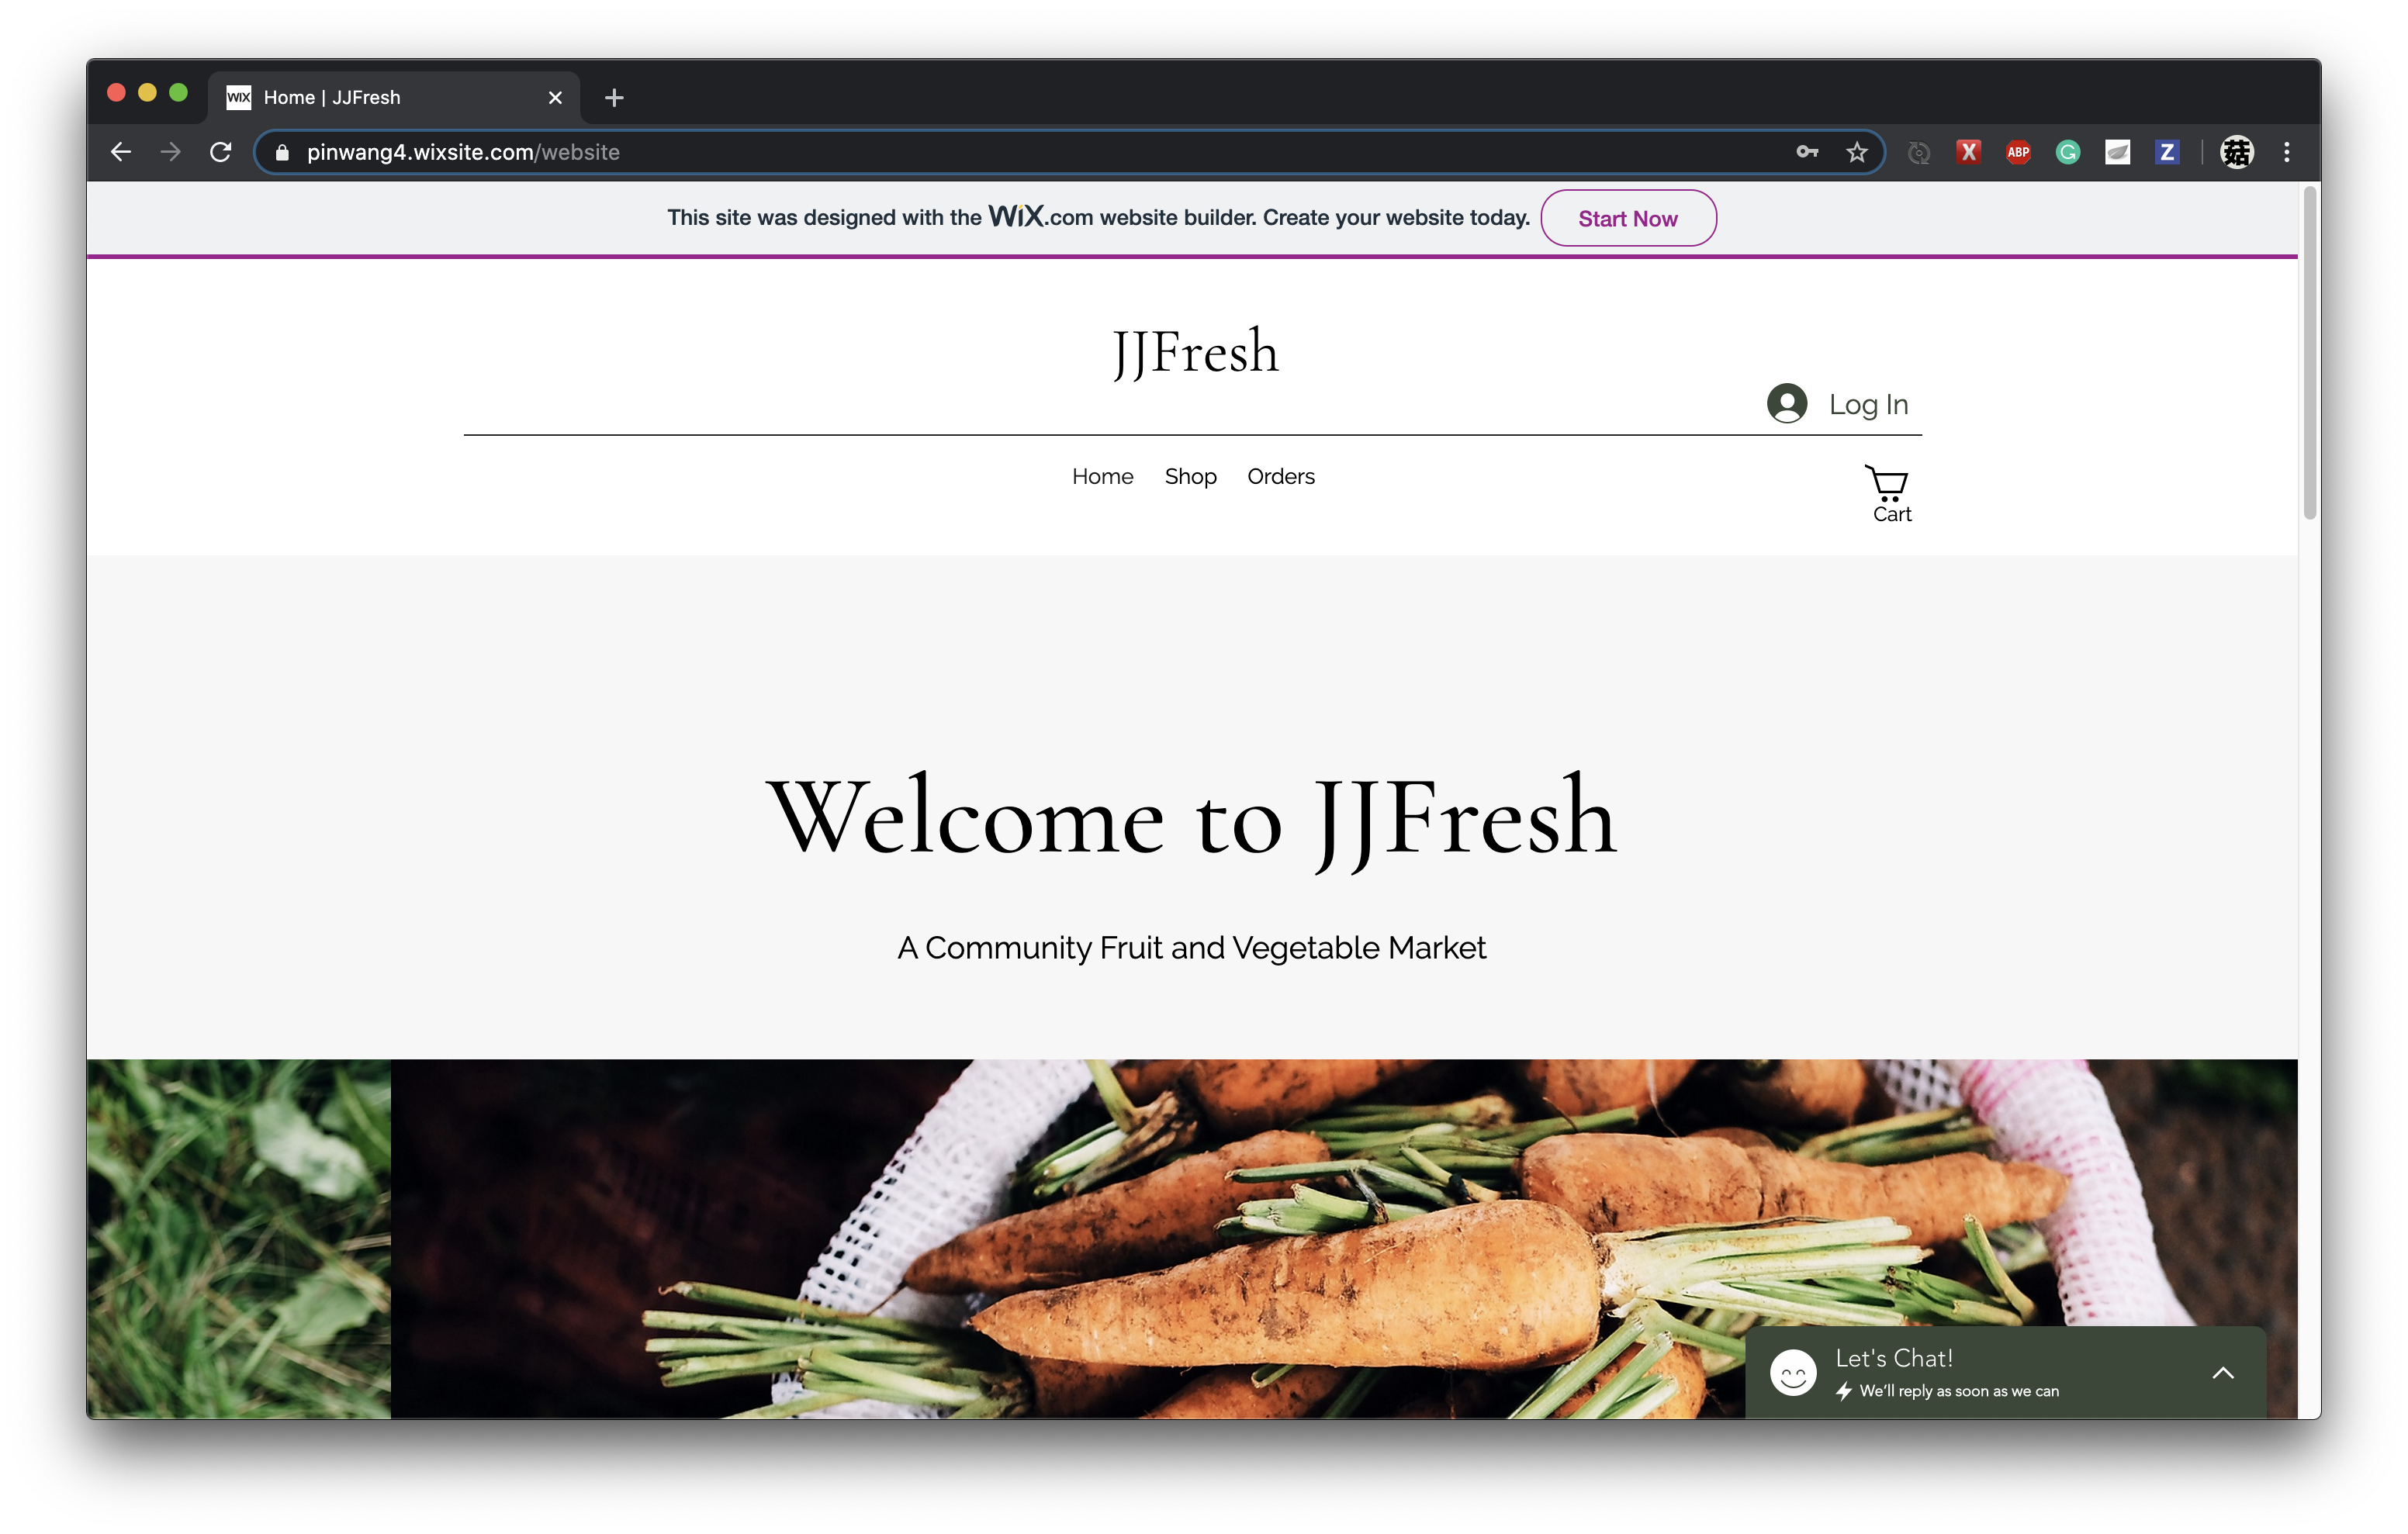
\includegraphics[width=\textwidth]{Figures/homepage.png}
\caption{Home page}
\label{fig:homepage}
\end{figure}

\clearpage
\section*{Login Page}
This page can be entered by clicking ‘Log in’ or the blank avatar before log in. Users can input the username and password to log into their account. If this is the first time to see this website, customer can register an account by clicking ‘Sign Up’.
\begin{figure}[htp]
\centering
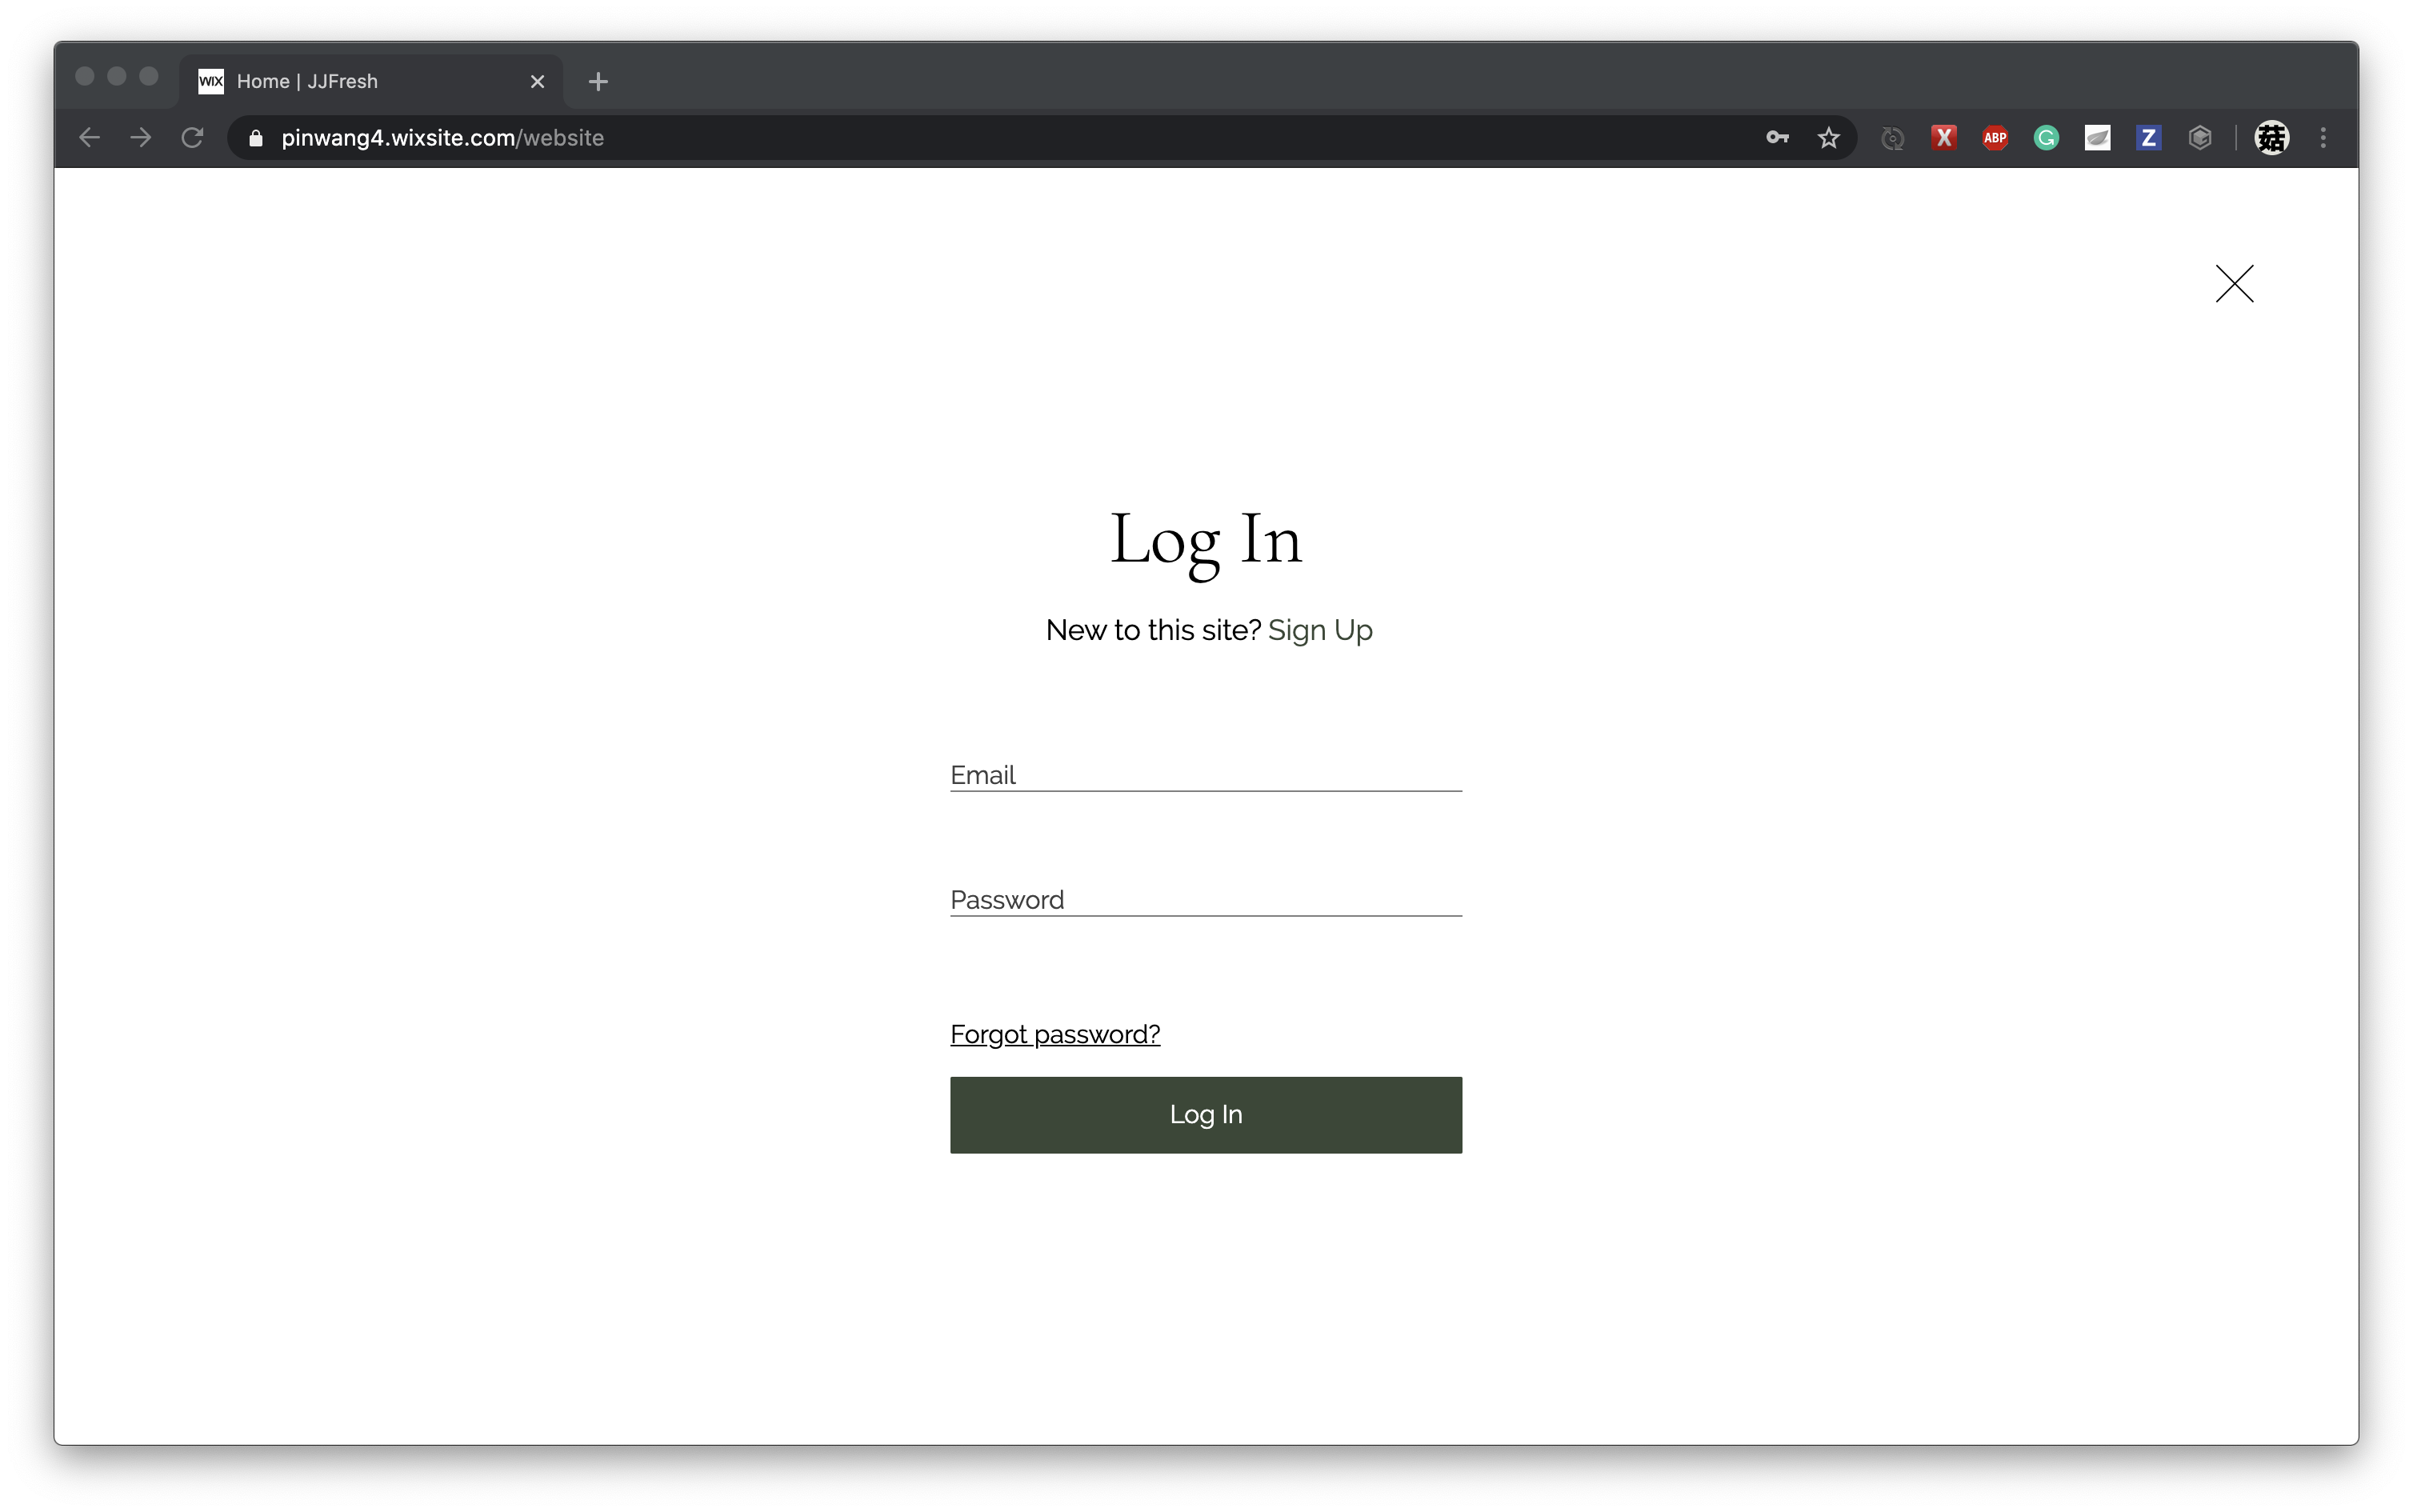
\includegraphics[width=\textwidth]{Figures/login.png}
\caption{Login}
\label{fig:login}
\end{figure}

\clearpage
\section*{Sign Up Page}
User can input a username, a valid email, and a password to register an account. Clicking ‘Sign Up’ after inputting, an email will be sent to user’s email address and the account is signed up.
\begin{figure}[htp]
\centering
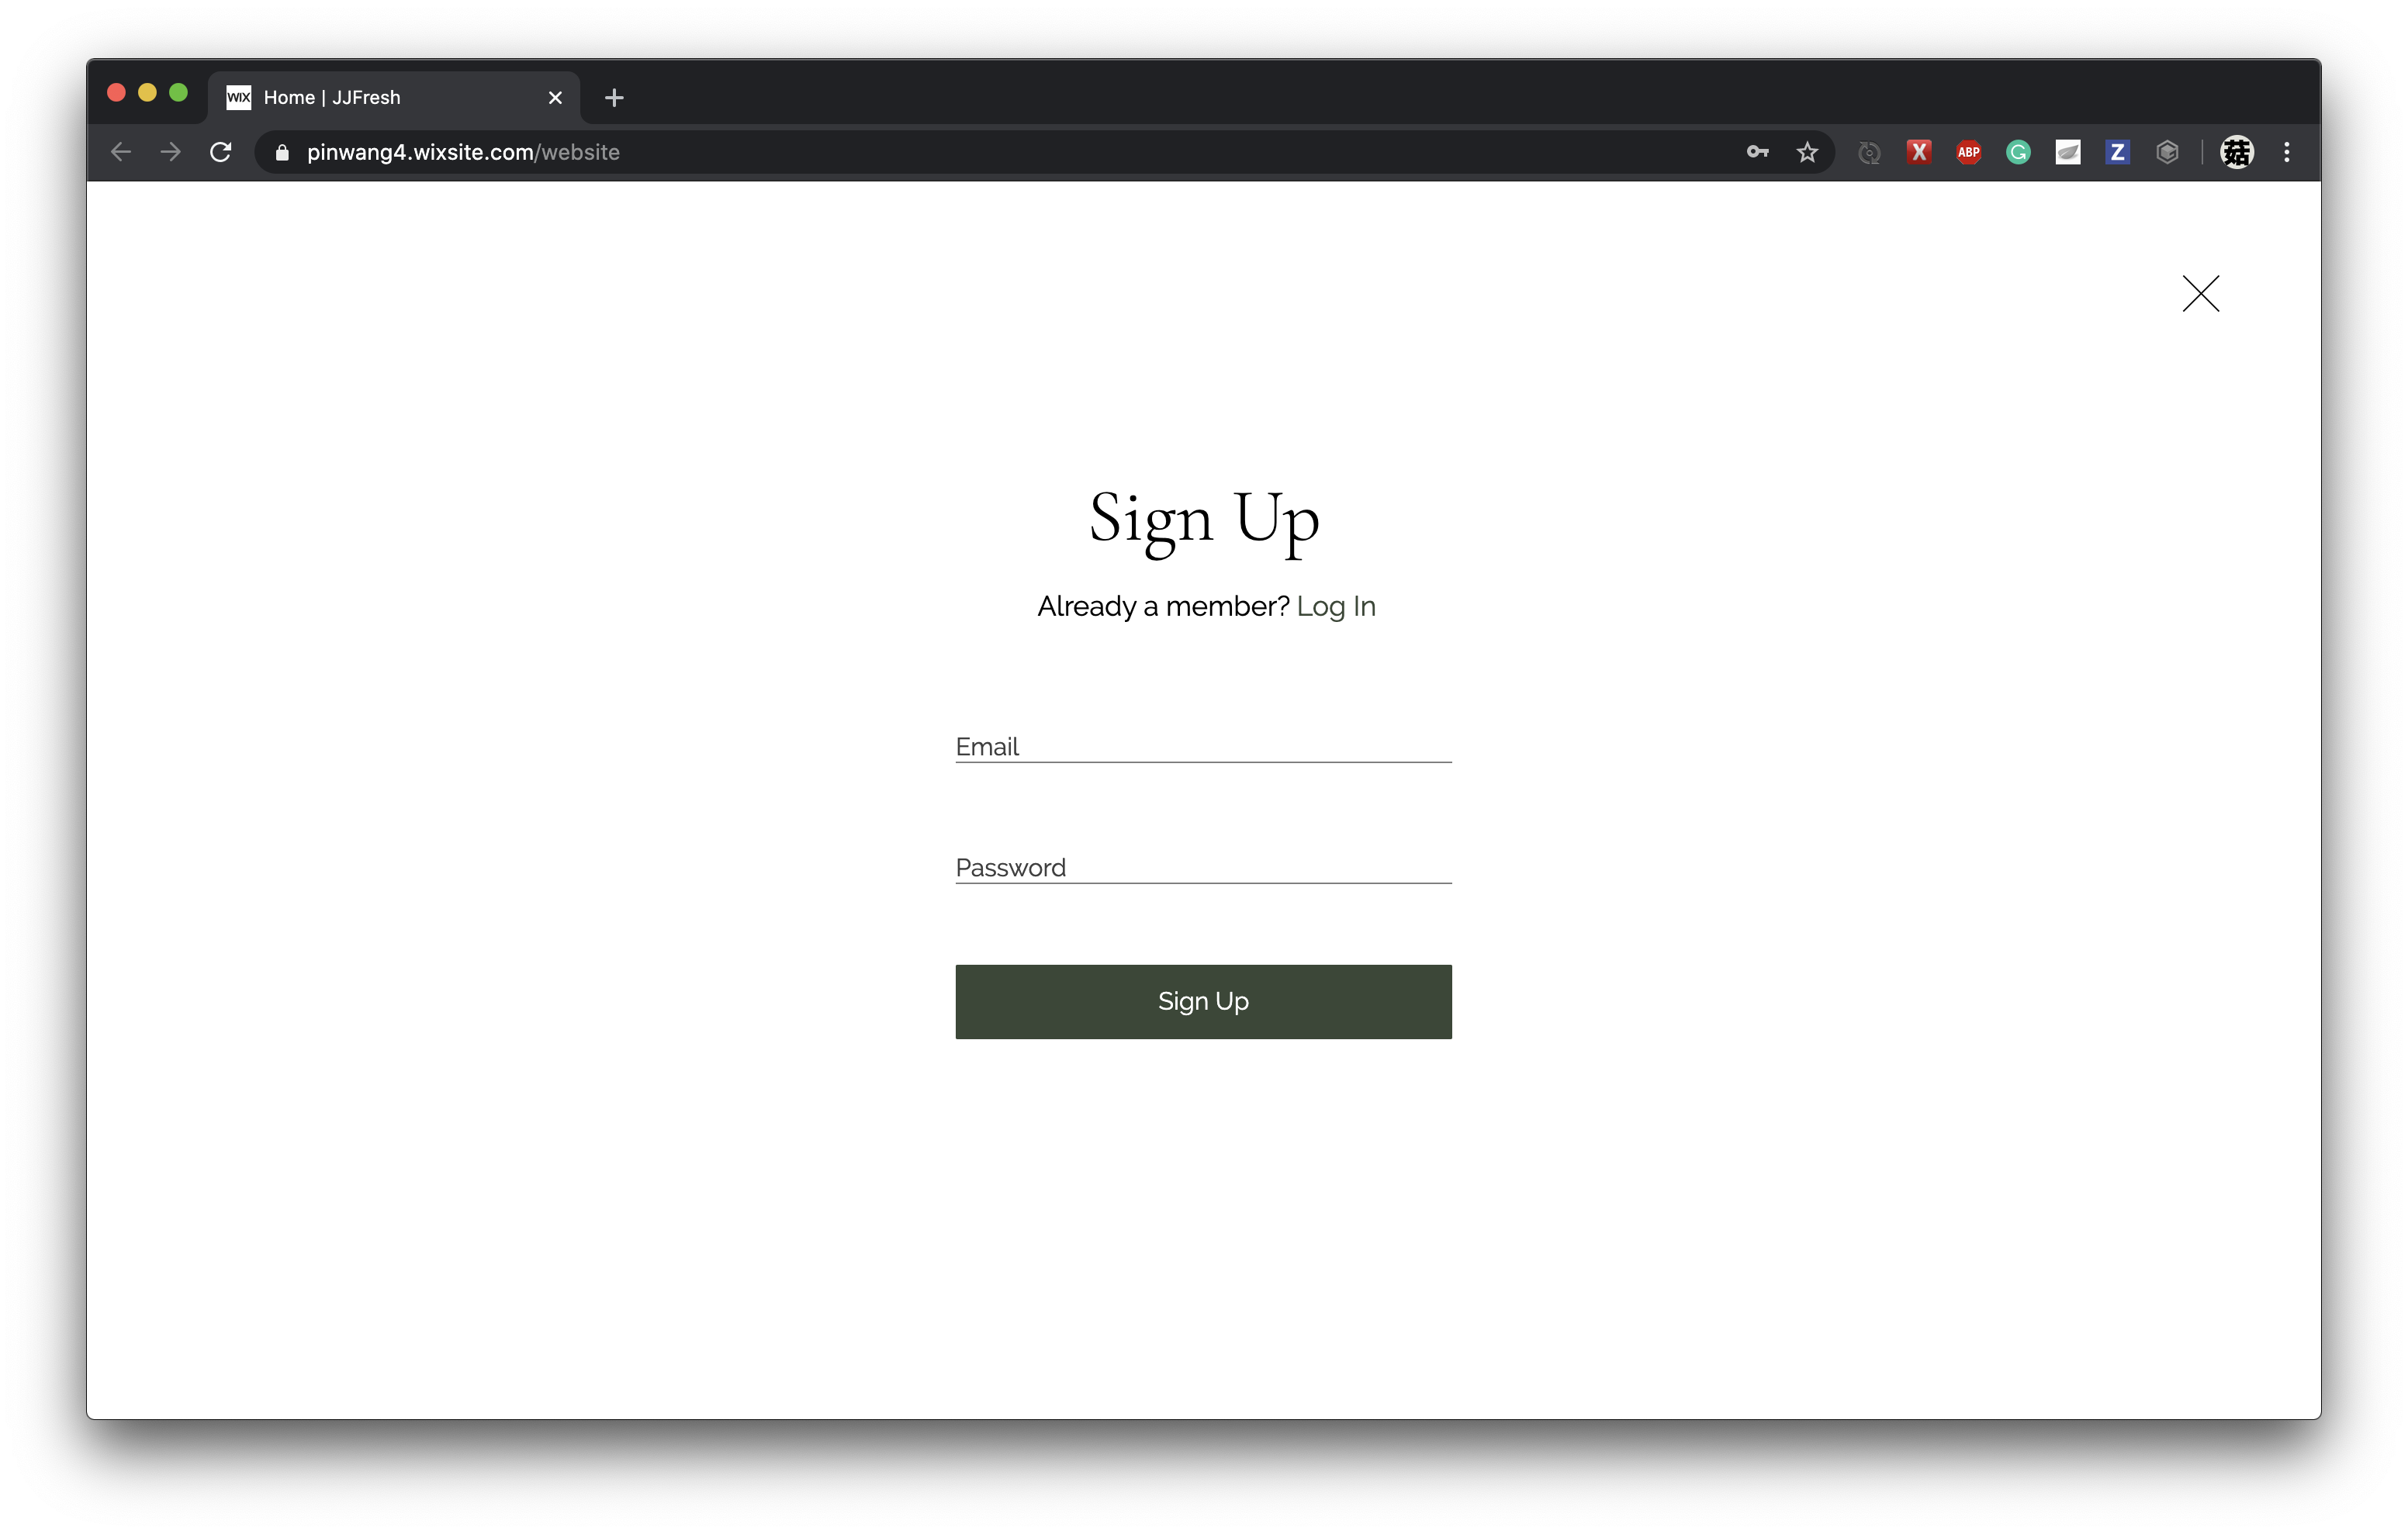
\includegraphics[width=\textwidth]{Figures/signup.png}
\caption{Sign Up}
\label{fig:signup}
\end{figure}

\clearpage
\section*{Drop-down Menu}
In the drop-down menu, there are my account, my backup phones, my address and Log out. Click ‘My Account’ can enter the personal information page of user. User can change his/her information and update by clicking ‘Updated’ button in the bottom of page.
Click ‘My backup phones’ on the menu or under the nick name box of the user information page can enter the backup phones page. User can add or change the backup phones in there and update it by clicking ‘Update’.
Click ‘My Address’ on the menu or under the nick name box of the user information page can enter the address information page. User can add or edit the delivery address in there and update it by click ‘Update’. 
Users can log out their accounts by clicking ‘Log Out’ on the menu.
\begin{figure}[htp]
\centering
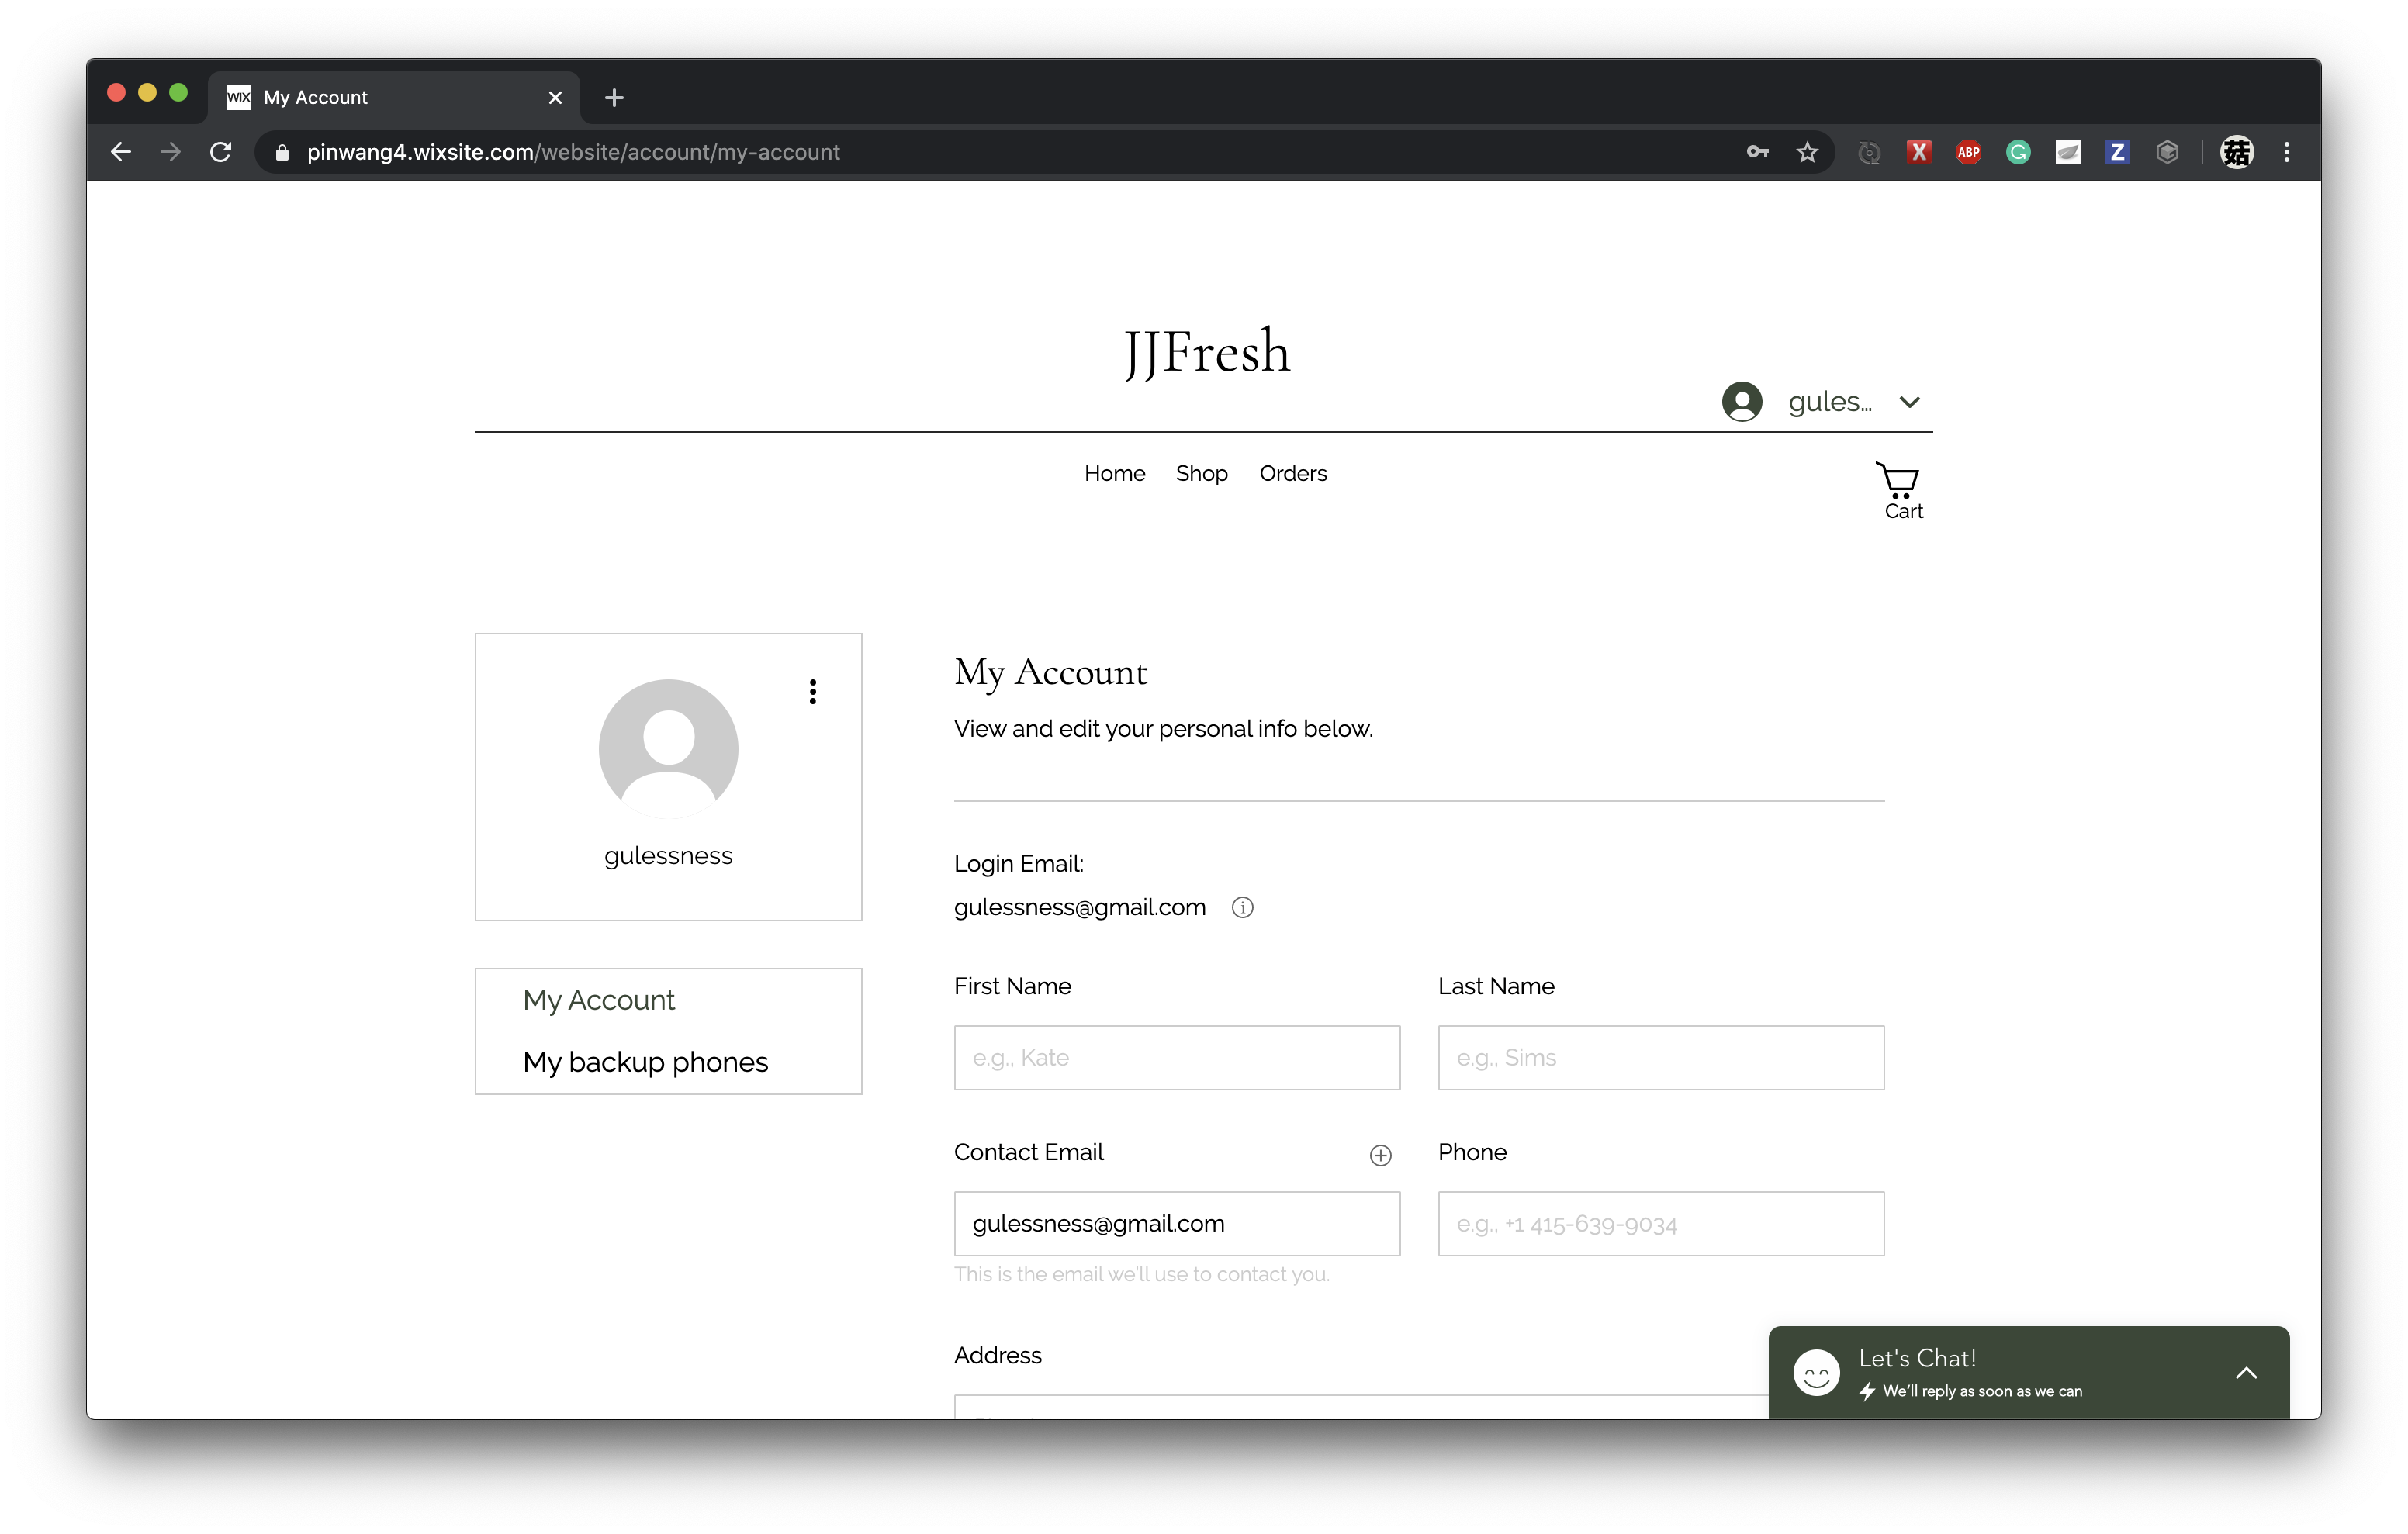
\includegraphics[width=\textwidth]{Figures/dropdown.png}
\caption{Drop-down Menu}
\label{fig:dropdown}
\end{figure}

\clearpage
\section*{Product Menu}
This page shows the product menu of JJFresh online store. In the initial stage, JJFresh can only provide 3 type of products, mixed fruit and vegetable box, vegetable box and fruit box. Users can check the detail of the products by clicking the corresponding button ‘View Details’.
\begin{figure}[htp]
\centering
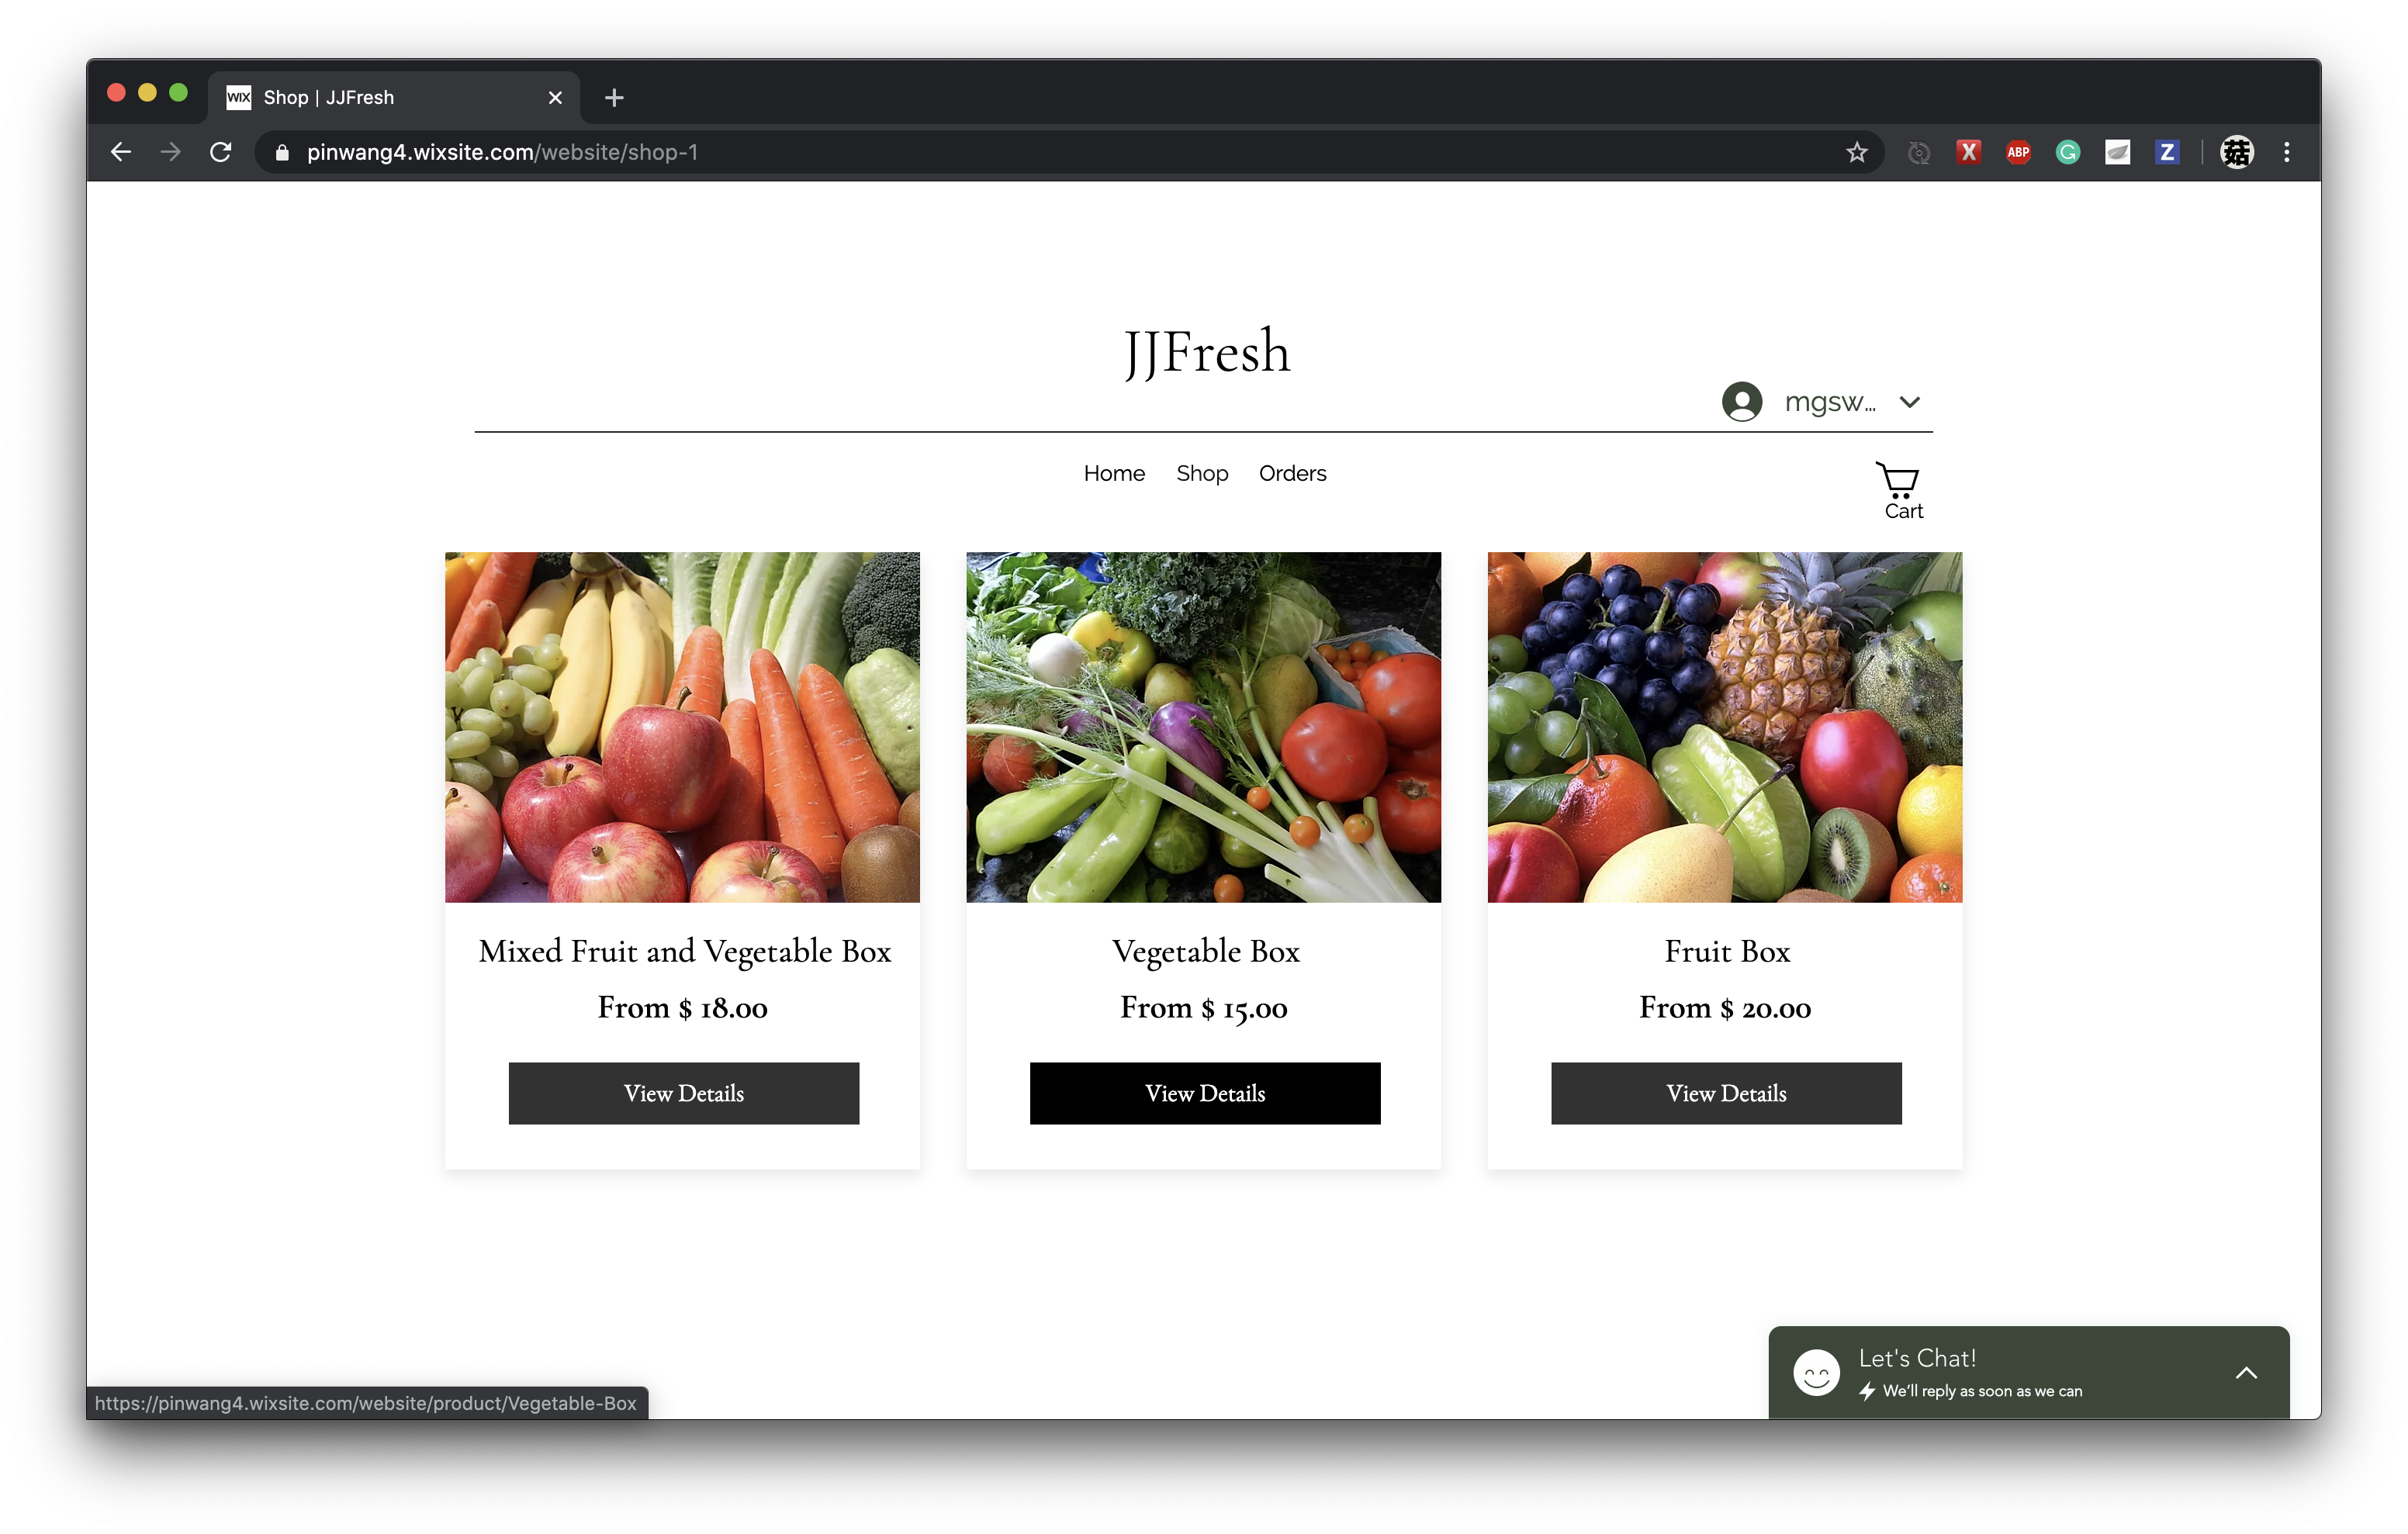
\includegraphics[width=\textwidth]{Figures/productMenu.png}
\caption{Screenshot of Product Menu }
\label{fig:productMenu}
\end{figure}

\clearpage
\section*{To add product}
This page shows the detail of the product that user click it. User can select size and quantity of product, the price wil change automatically after selecting. User can click 'Add to Cart' to add selected products into cart.
\begin{figure}[htp]
\centering
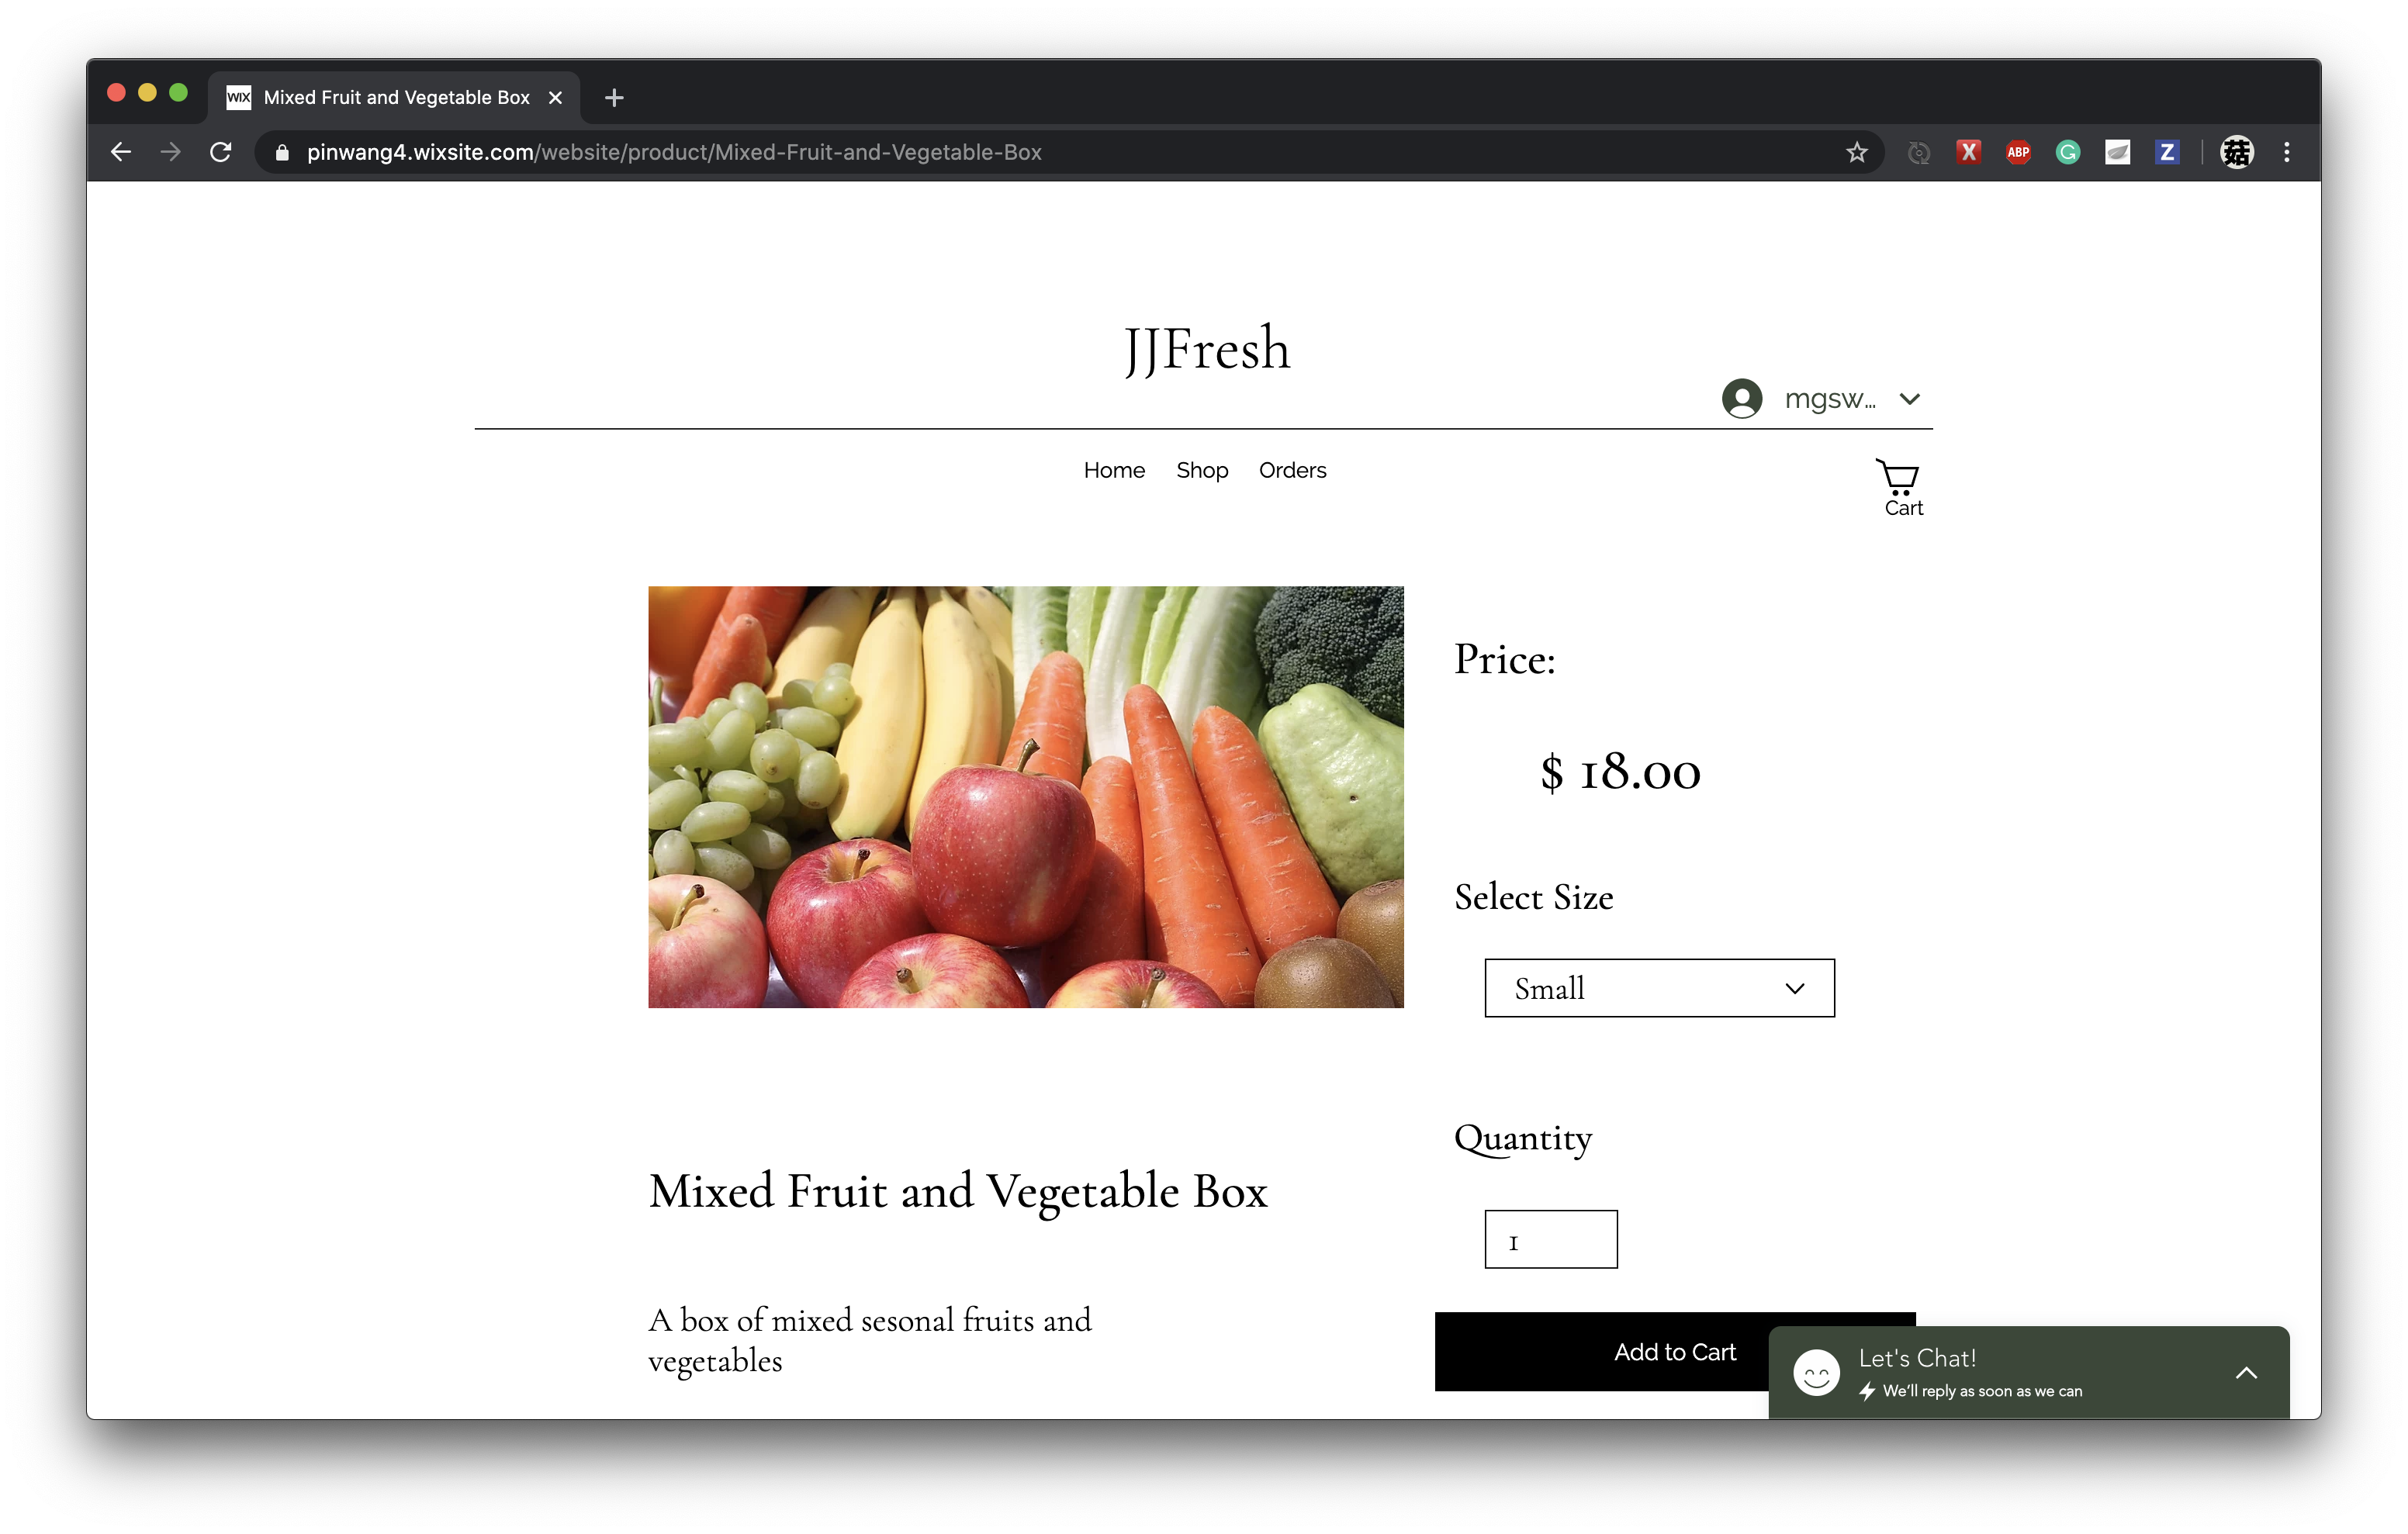
\includegraphics[width=\textwidth]{Figures/addProduct.png}
\caption{Screenshot of adding product}
\label{fig:addProduct}
\end{figure}

\clearpage
\section*{Shoping cart}
This little page just shows the list of products which were put into the cart.
\begin{figure}[htp]
\centering
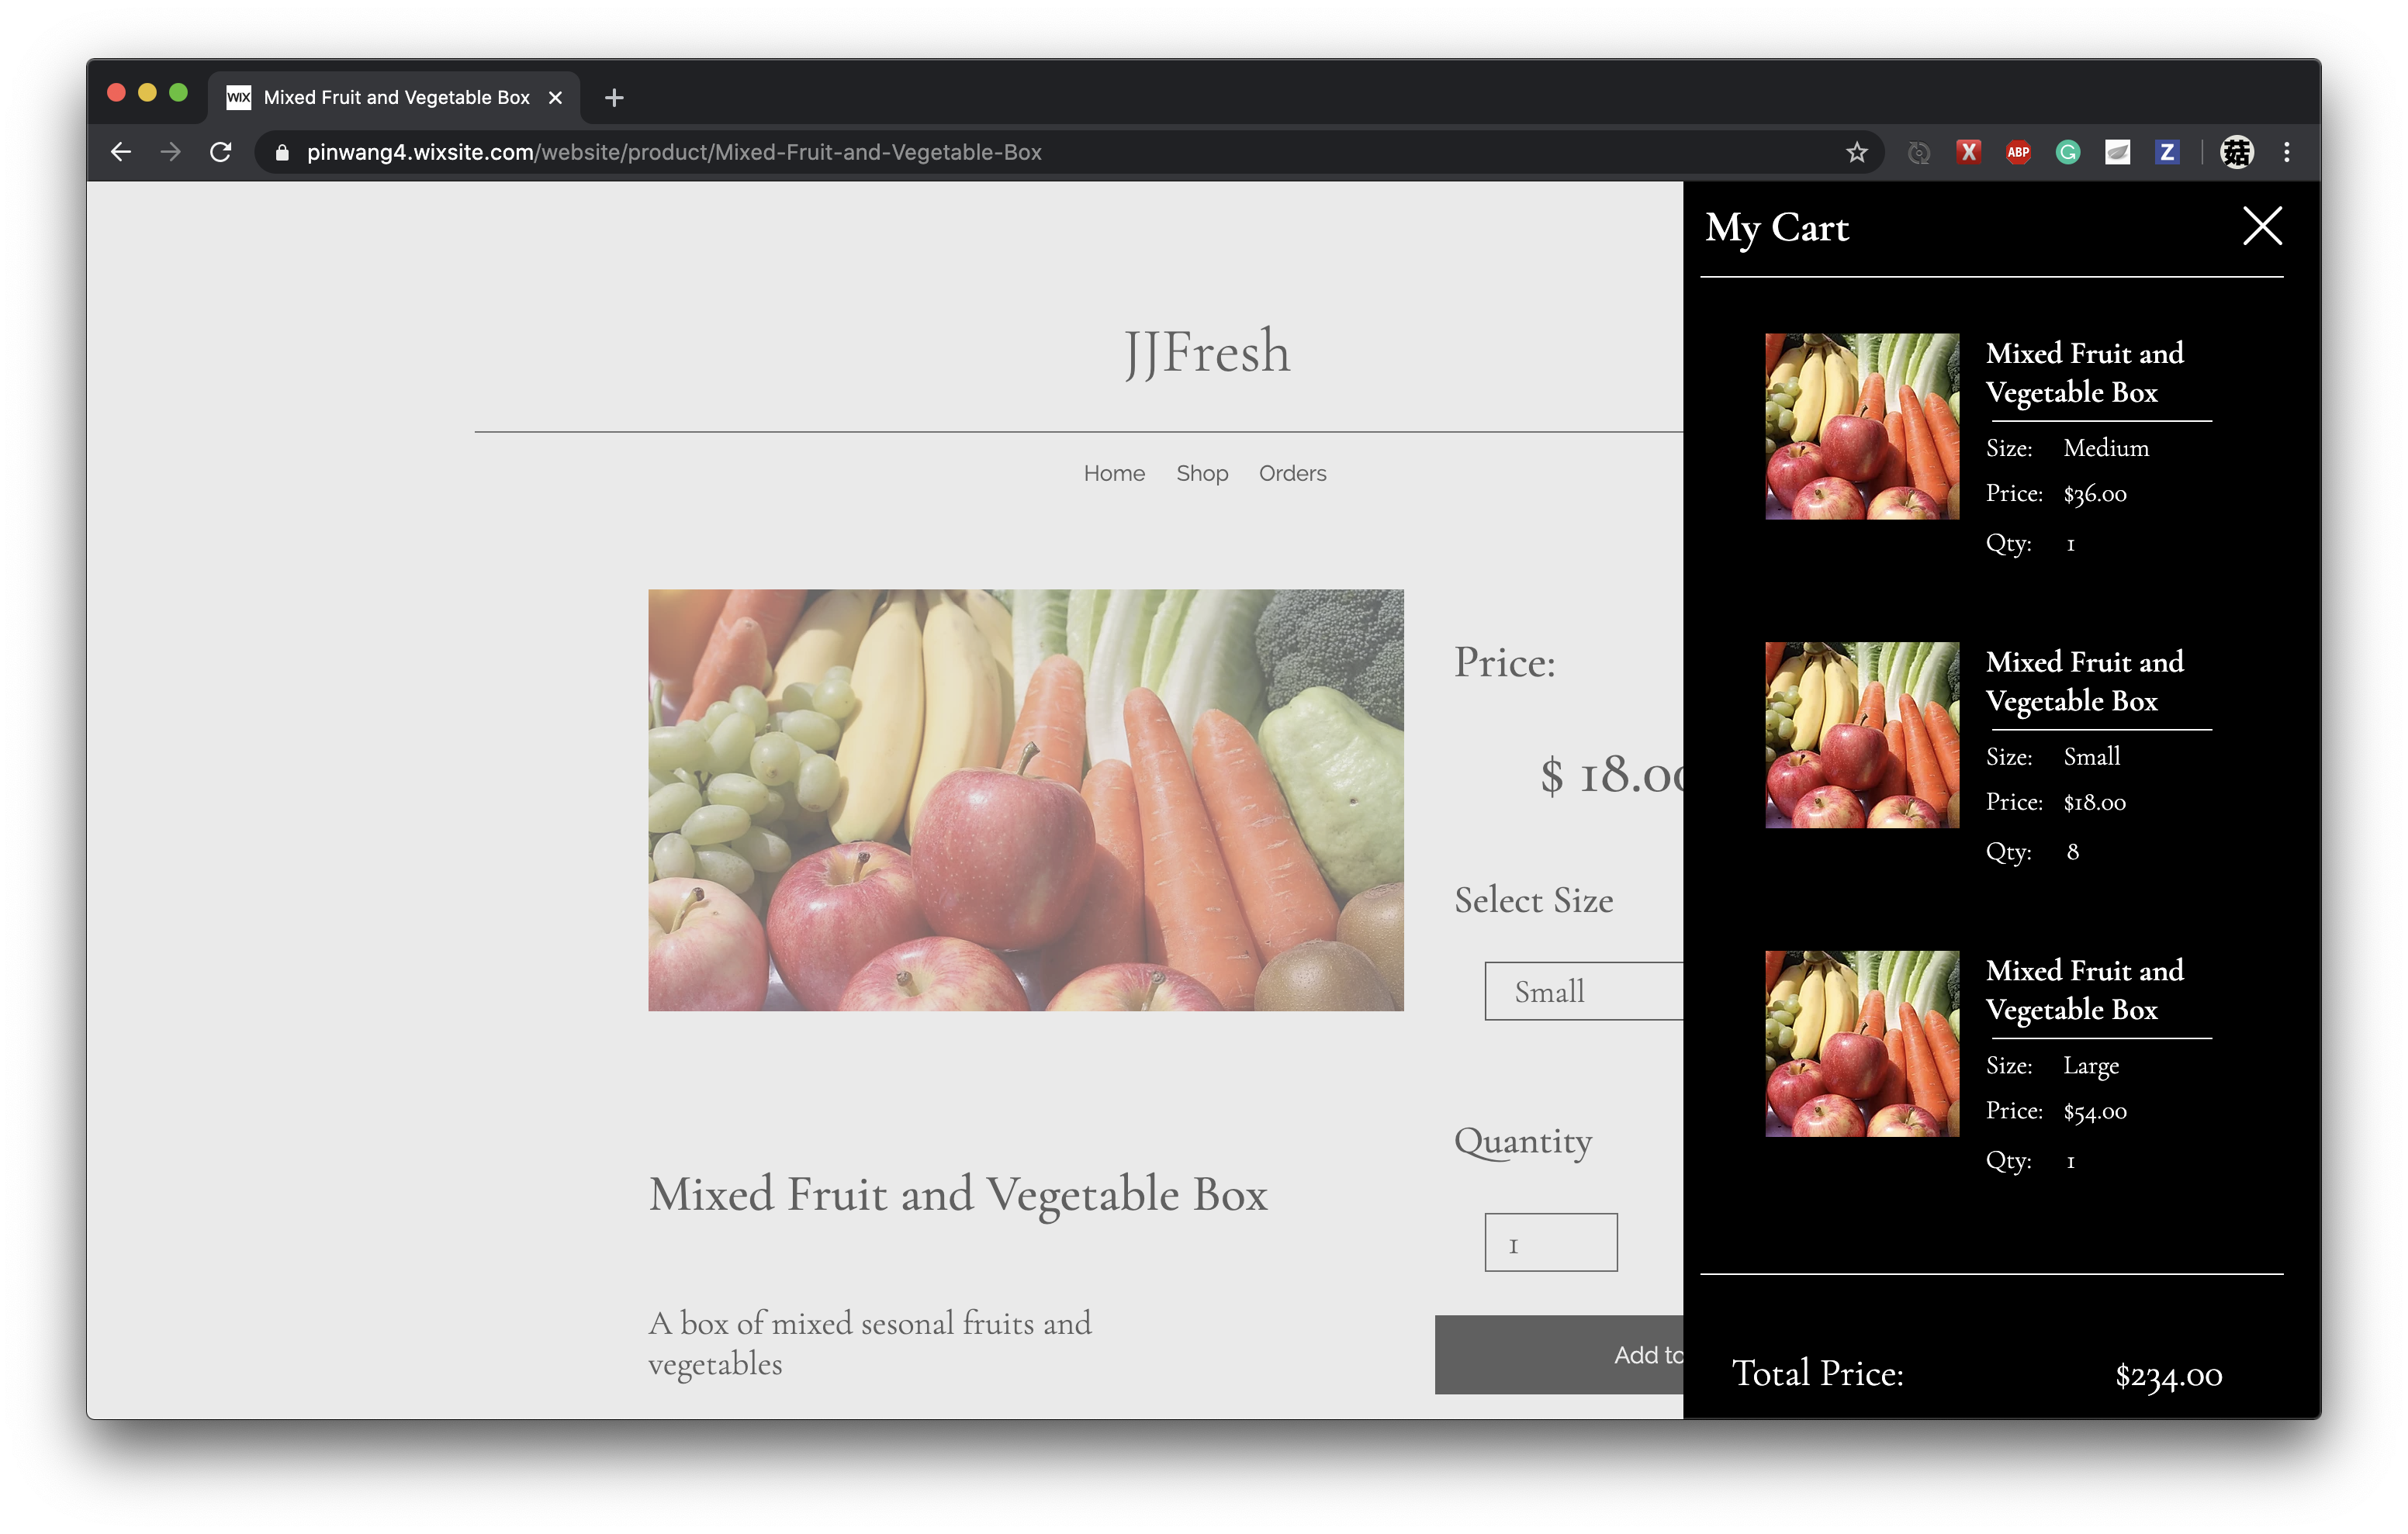
\includegraphics[width=\textwidth]{Figures/shoppingCart.png}
\caption{Screenshot of Shopping Cart}
\label{fig:shoppingCart}
\end{figure}

\clearpage
\section*{Check out page}
This page shows the list of products that user picking and the total price. Each product in the list has a check button ‘BUY IT’. If user check it, then the product would be bought, and its price would be added to the total price.
\begin{figure}[htp]
\centering
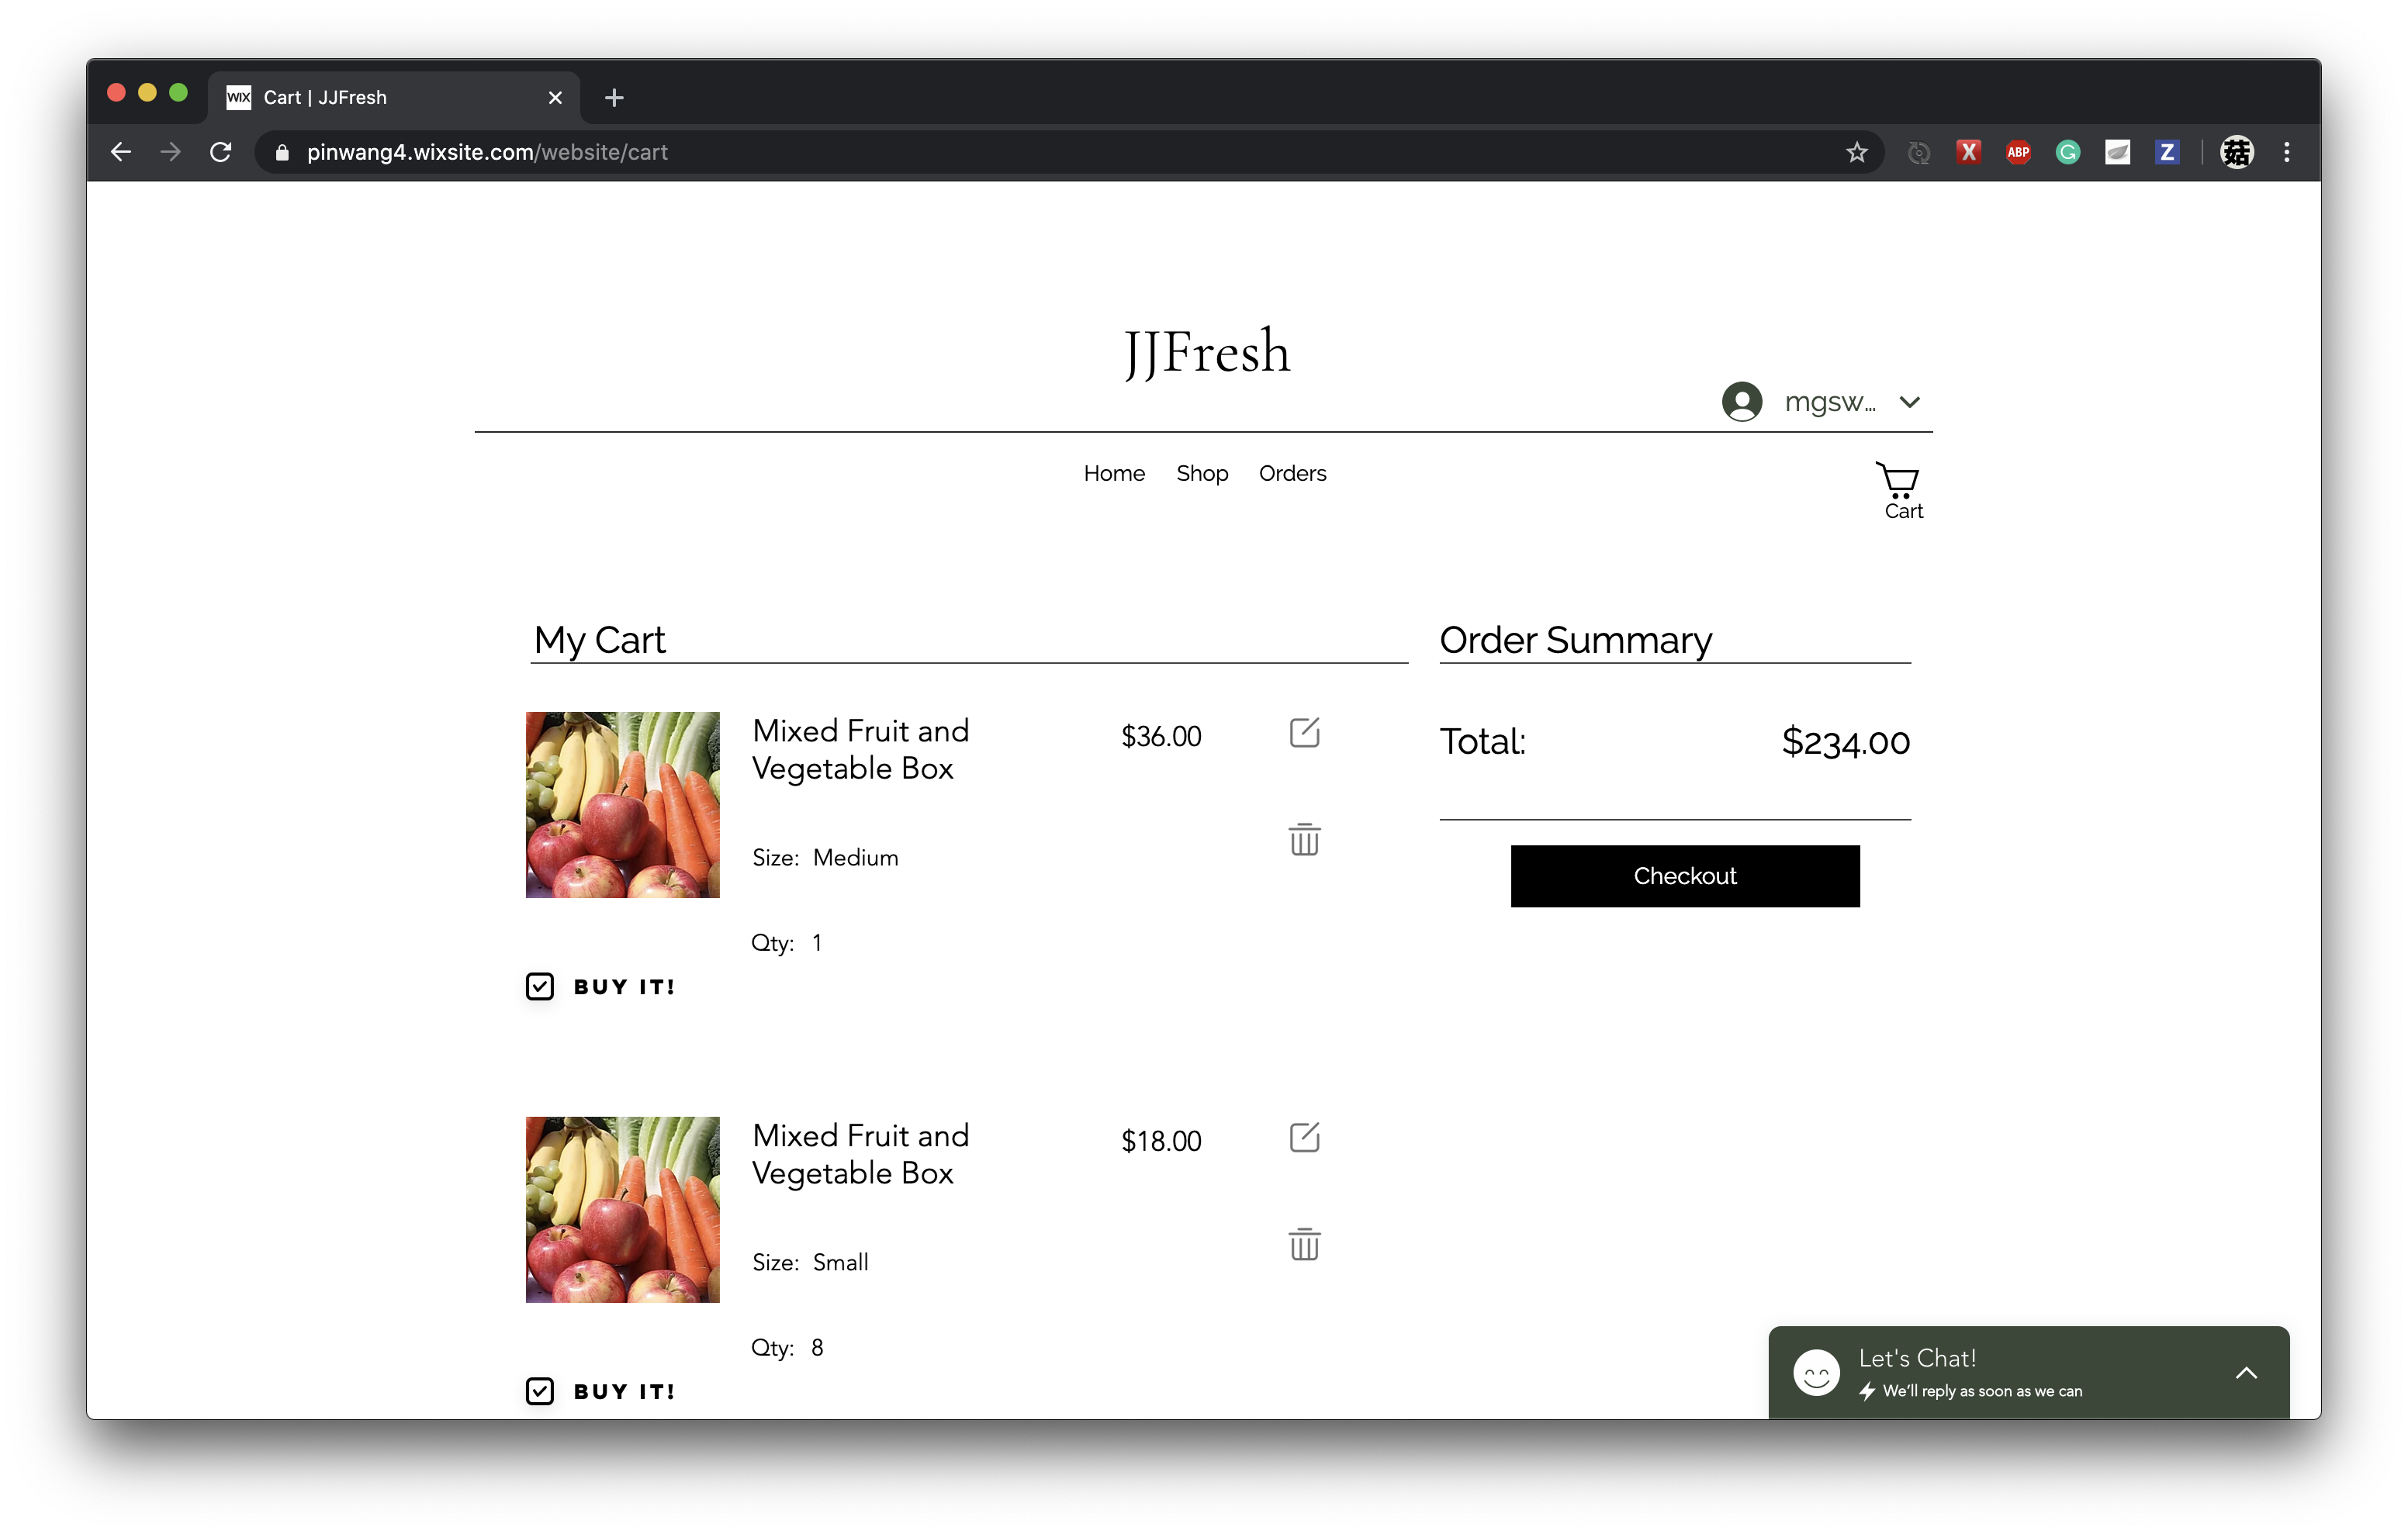
\includegraphics[width=\textwidth]{Figures/checkoutPage.png}
\caption{Screenshot of Checkout page}
\label{fig:checkoutPage}
\end{figure}


\clearpage
\section*{Delivery Date Selection page}
In this page, users can place a new booking order by selecting the appropriate date and time and filling the delivery address form. After filling all blanks, click ‘Place Order’ and the delivery order is done.
\begin{figure}[htp]
\centering
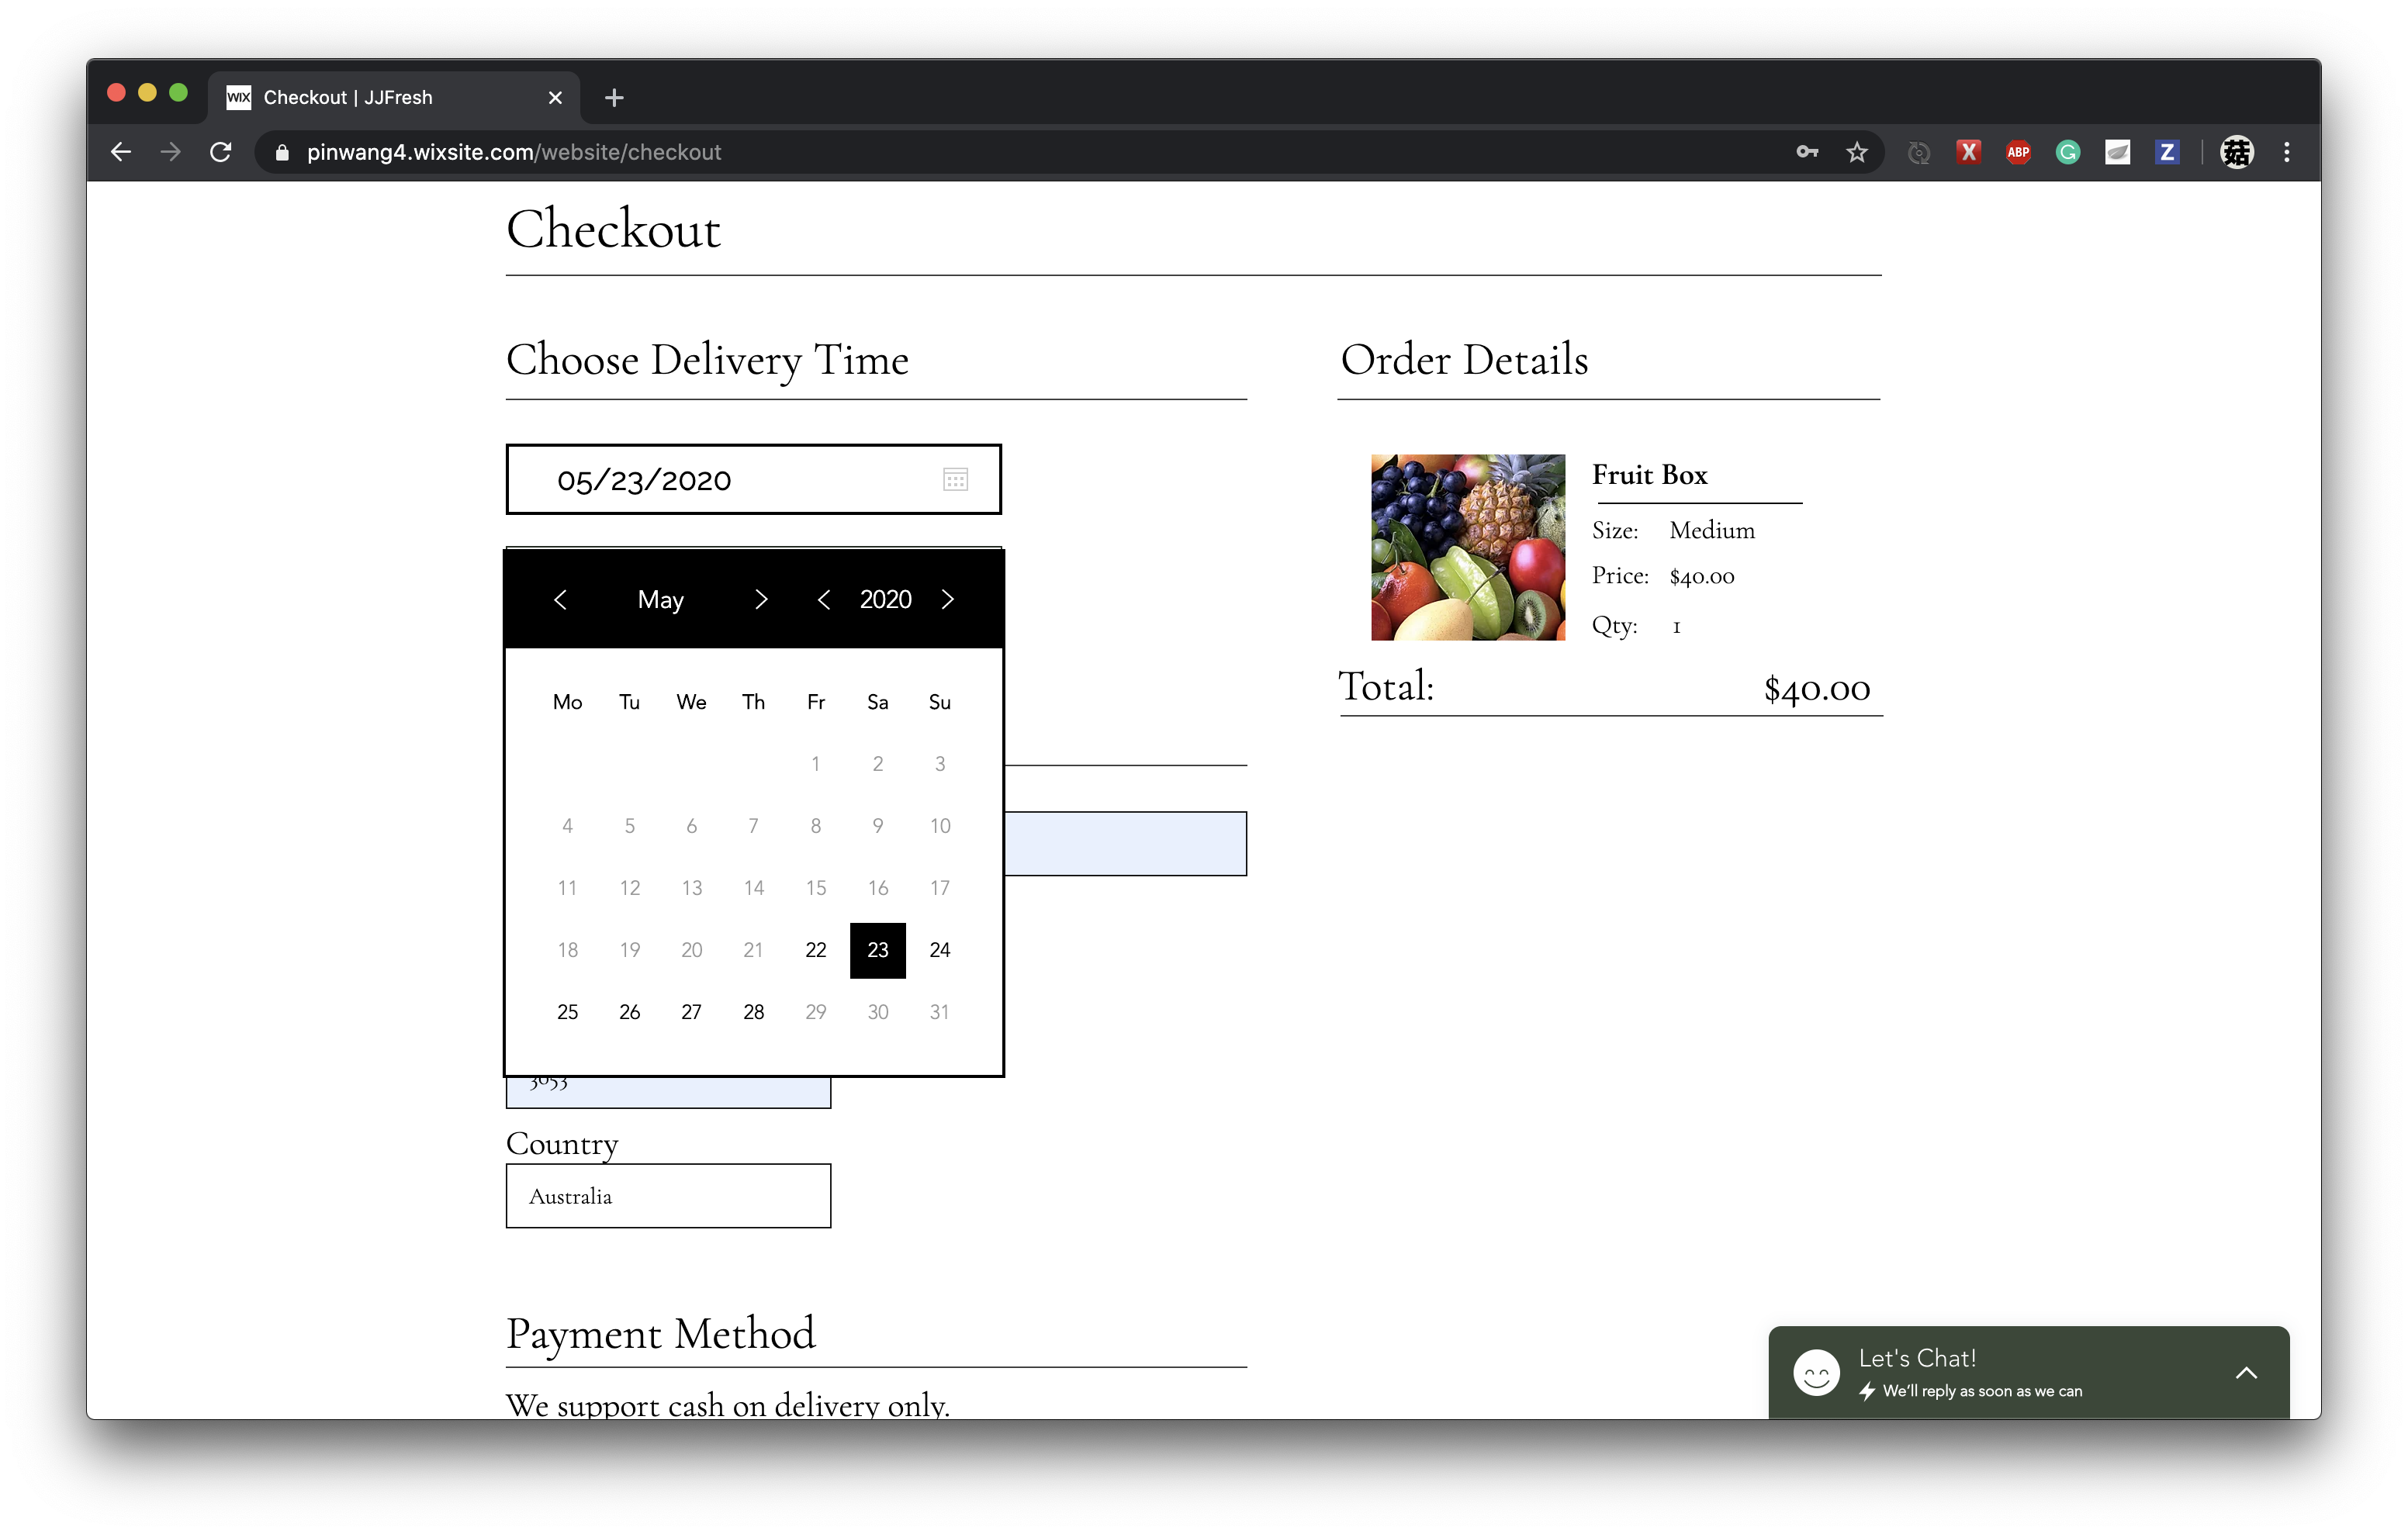
\includegraphics[width=\textwidth]{Figures/dateSelect.png}
\caption{Screenshot of Delivery Date Select}
\label{fig:dateSelect}
\end{figure}

\clearpage
\section*{Cancel orders page}
If users want to cancel their orders, they can click ‘Orders’ to enter the cancel orders page. In this page, user can see all the orders they have placed. They just need to click the ‘Cancel’ near the orders they want to cancel.
\begin{figure}[htp]
\centering
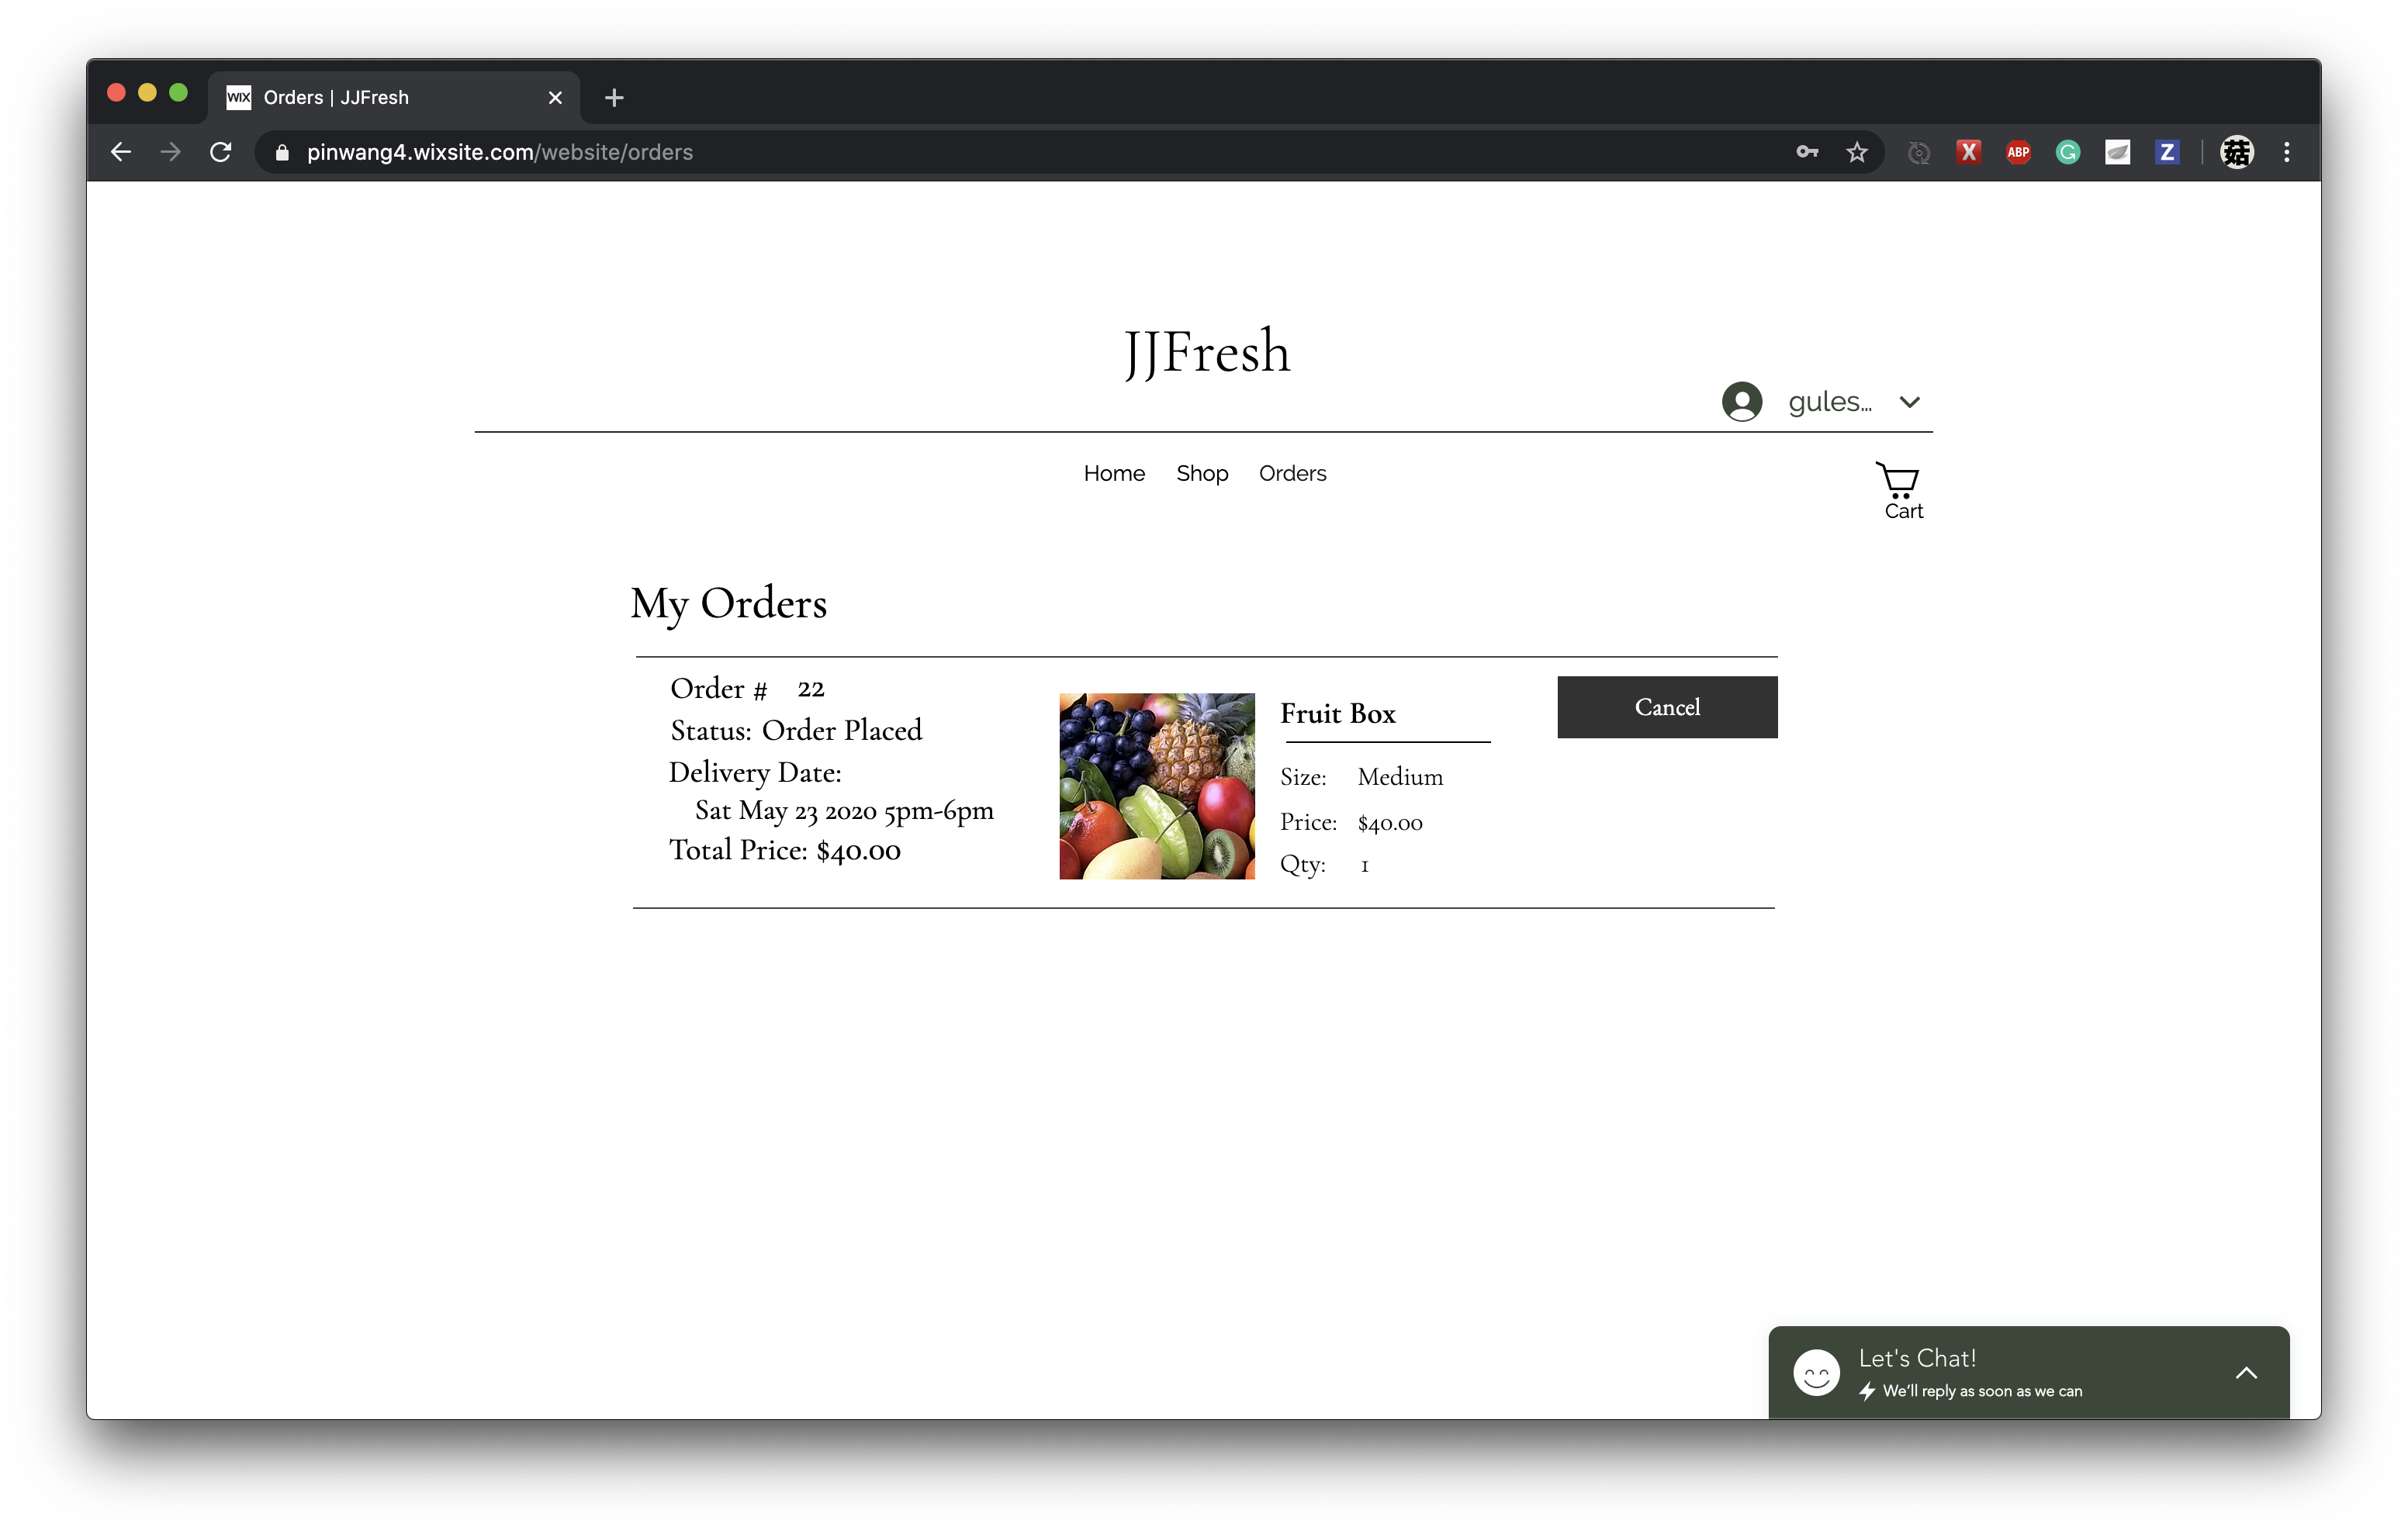
\includegraphics[width=\textwidth]{Figures/customerOrder.png}
\caption{Screenshot of Customers order management page}
\label{fig:customerOrder}
\end{figure}

\clearpage
\section*{Confirmed email}
Confirm email is used to confirm user’s orders have been confirmed by JJFresh or has been cancelled and user’s delivery orders have been finished.
\begin{figure}[htp]
\centering
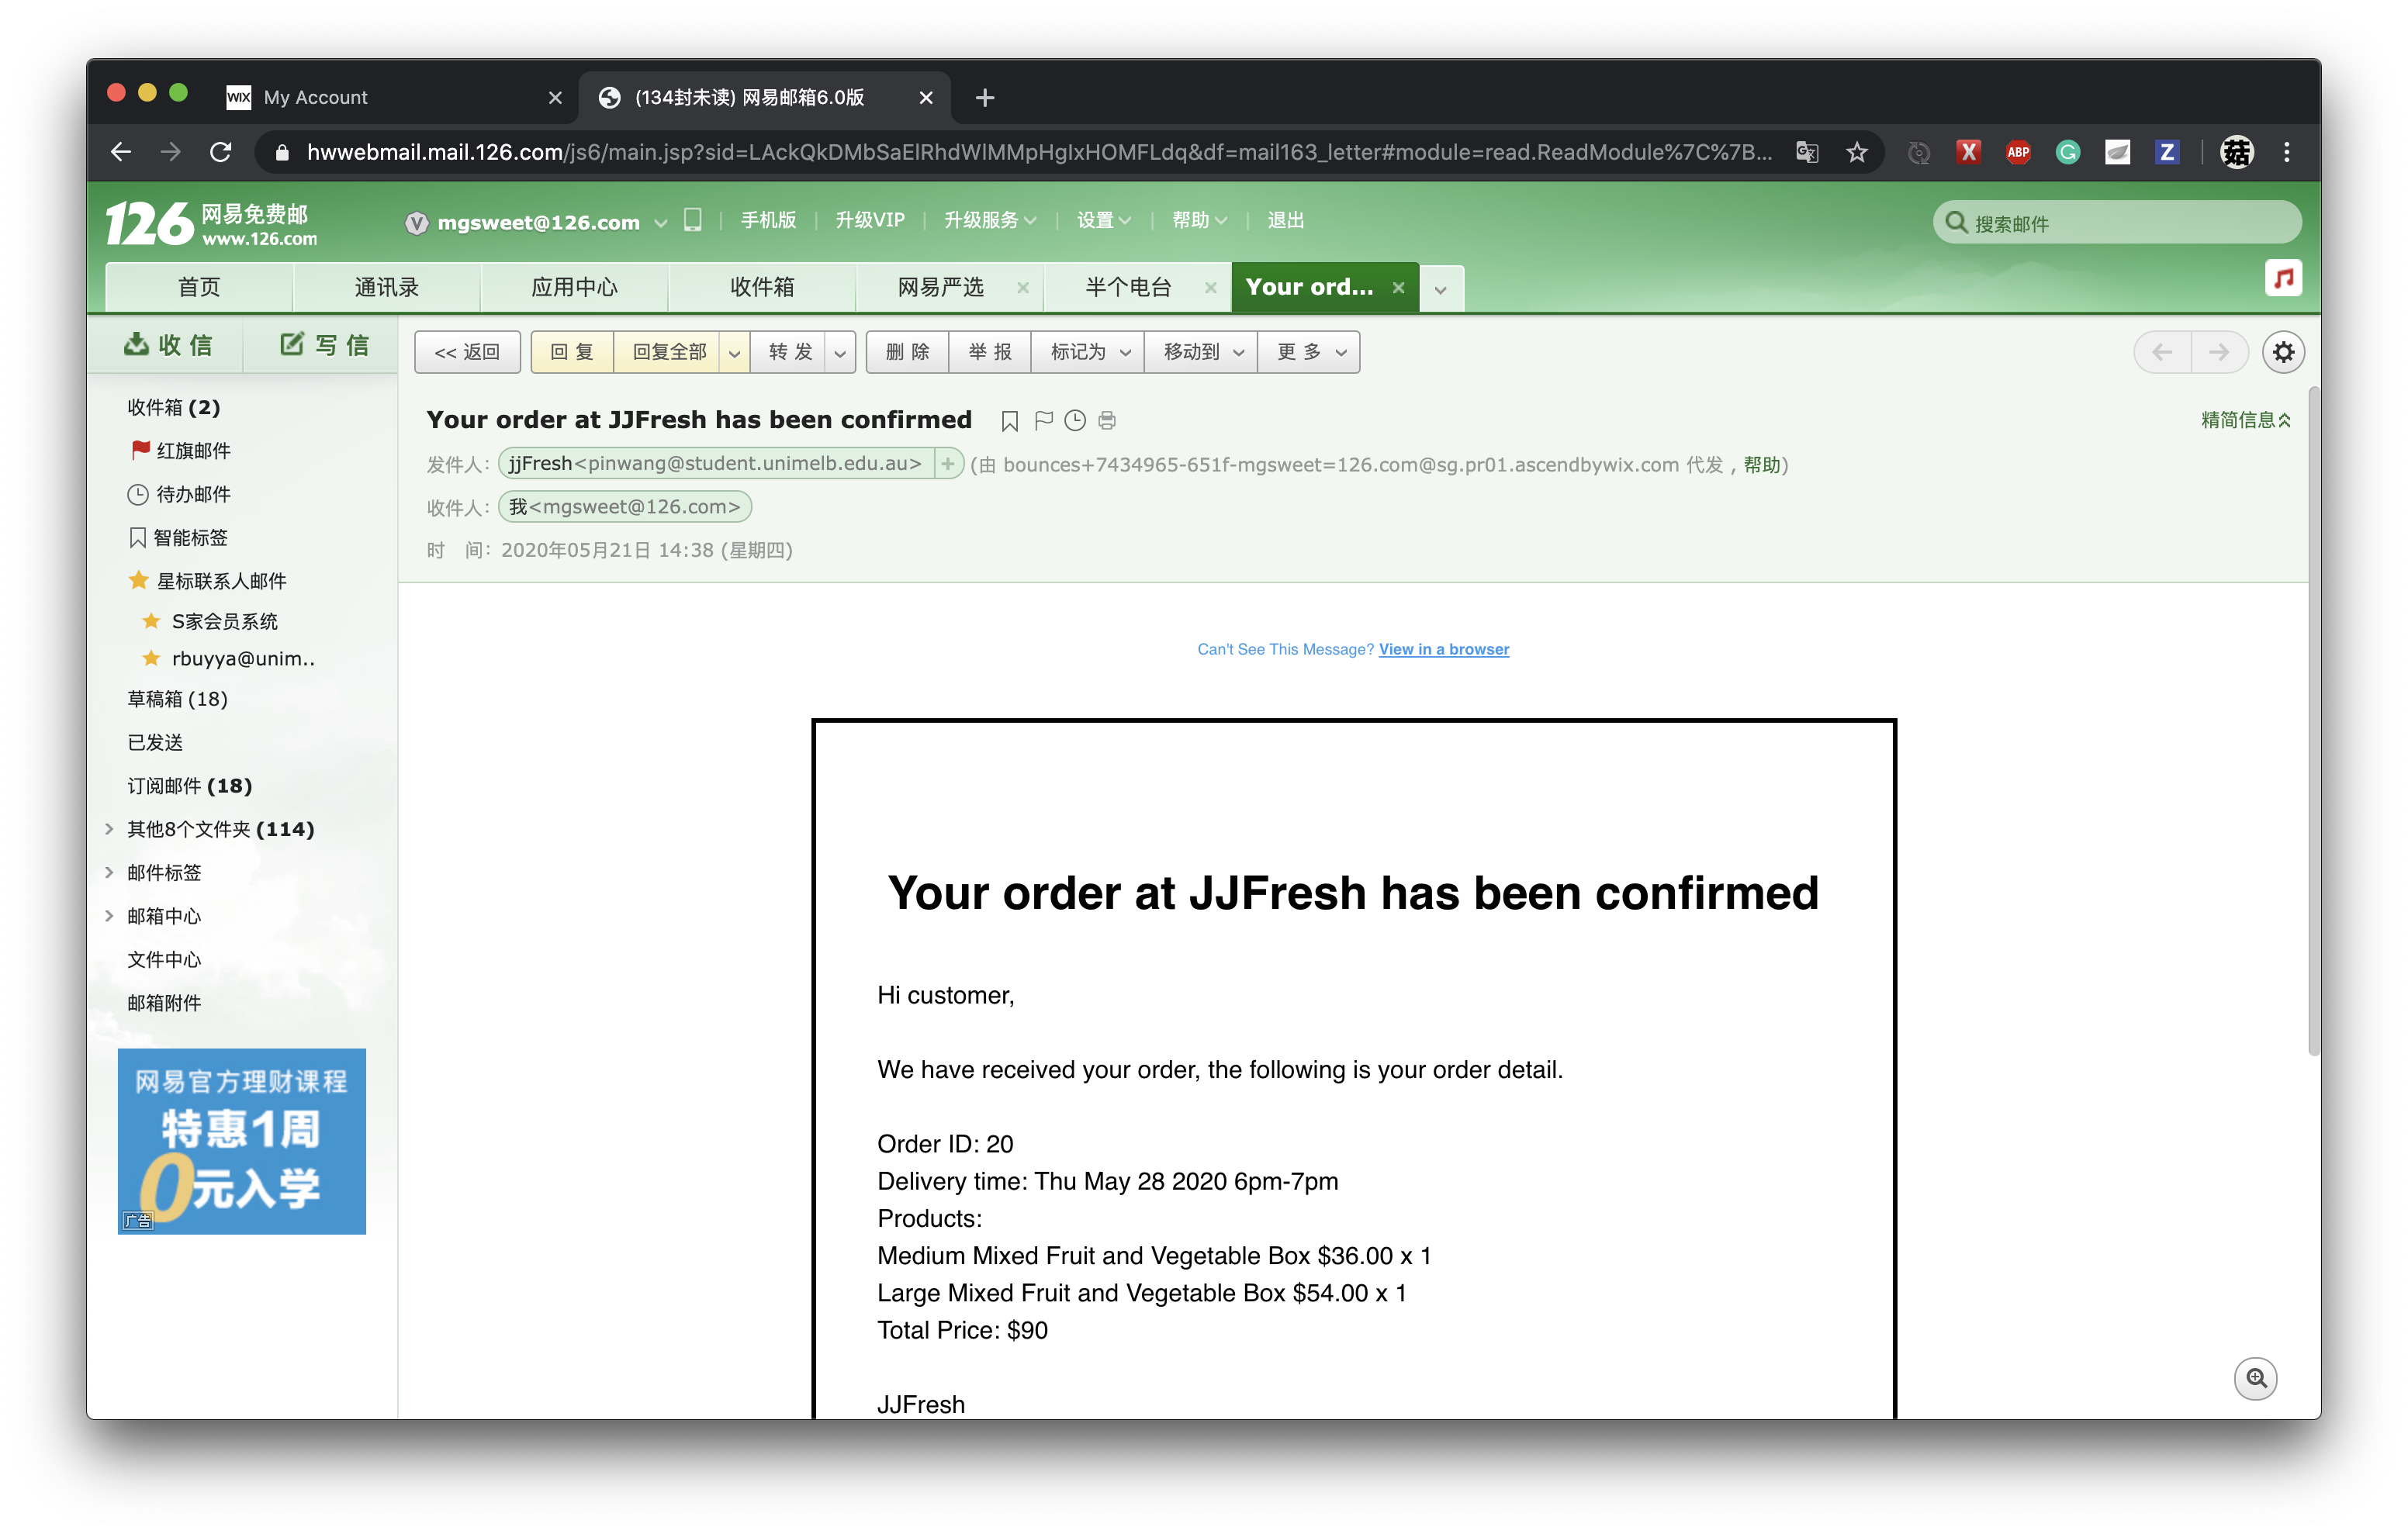
\includegraphics[width=\textwidth]{Figures/confirmedEmail.png}
\caption{Screenshot of confirmed email}
\label{fig:confirmedEmail}
\end{figure}

\clearpage
\section*{Admin manage products page}
This page can be entered by click ‘Product Management’. Jess and James can manage all the products in this page with an admin account. If they want to adjust the related information of a product, they just need to click ‘Manage this product’ of the corresponding product. They can click ‘Delete this product’ to remove the corresponding product from the online store.
If Jessa and James want to add more products in the later stage, they can click ‘Add A Product’ to enter the page that adding information form of new product.
\begin{figure}[htp]
\centering
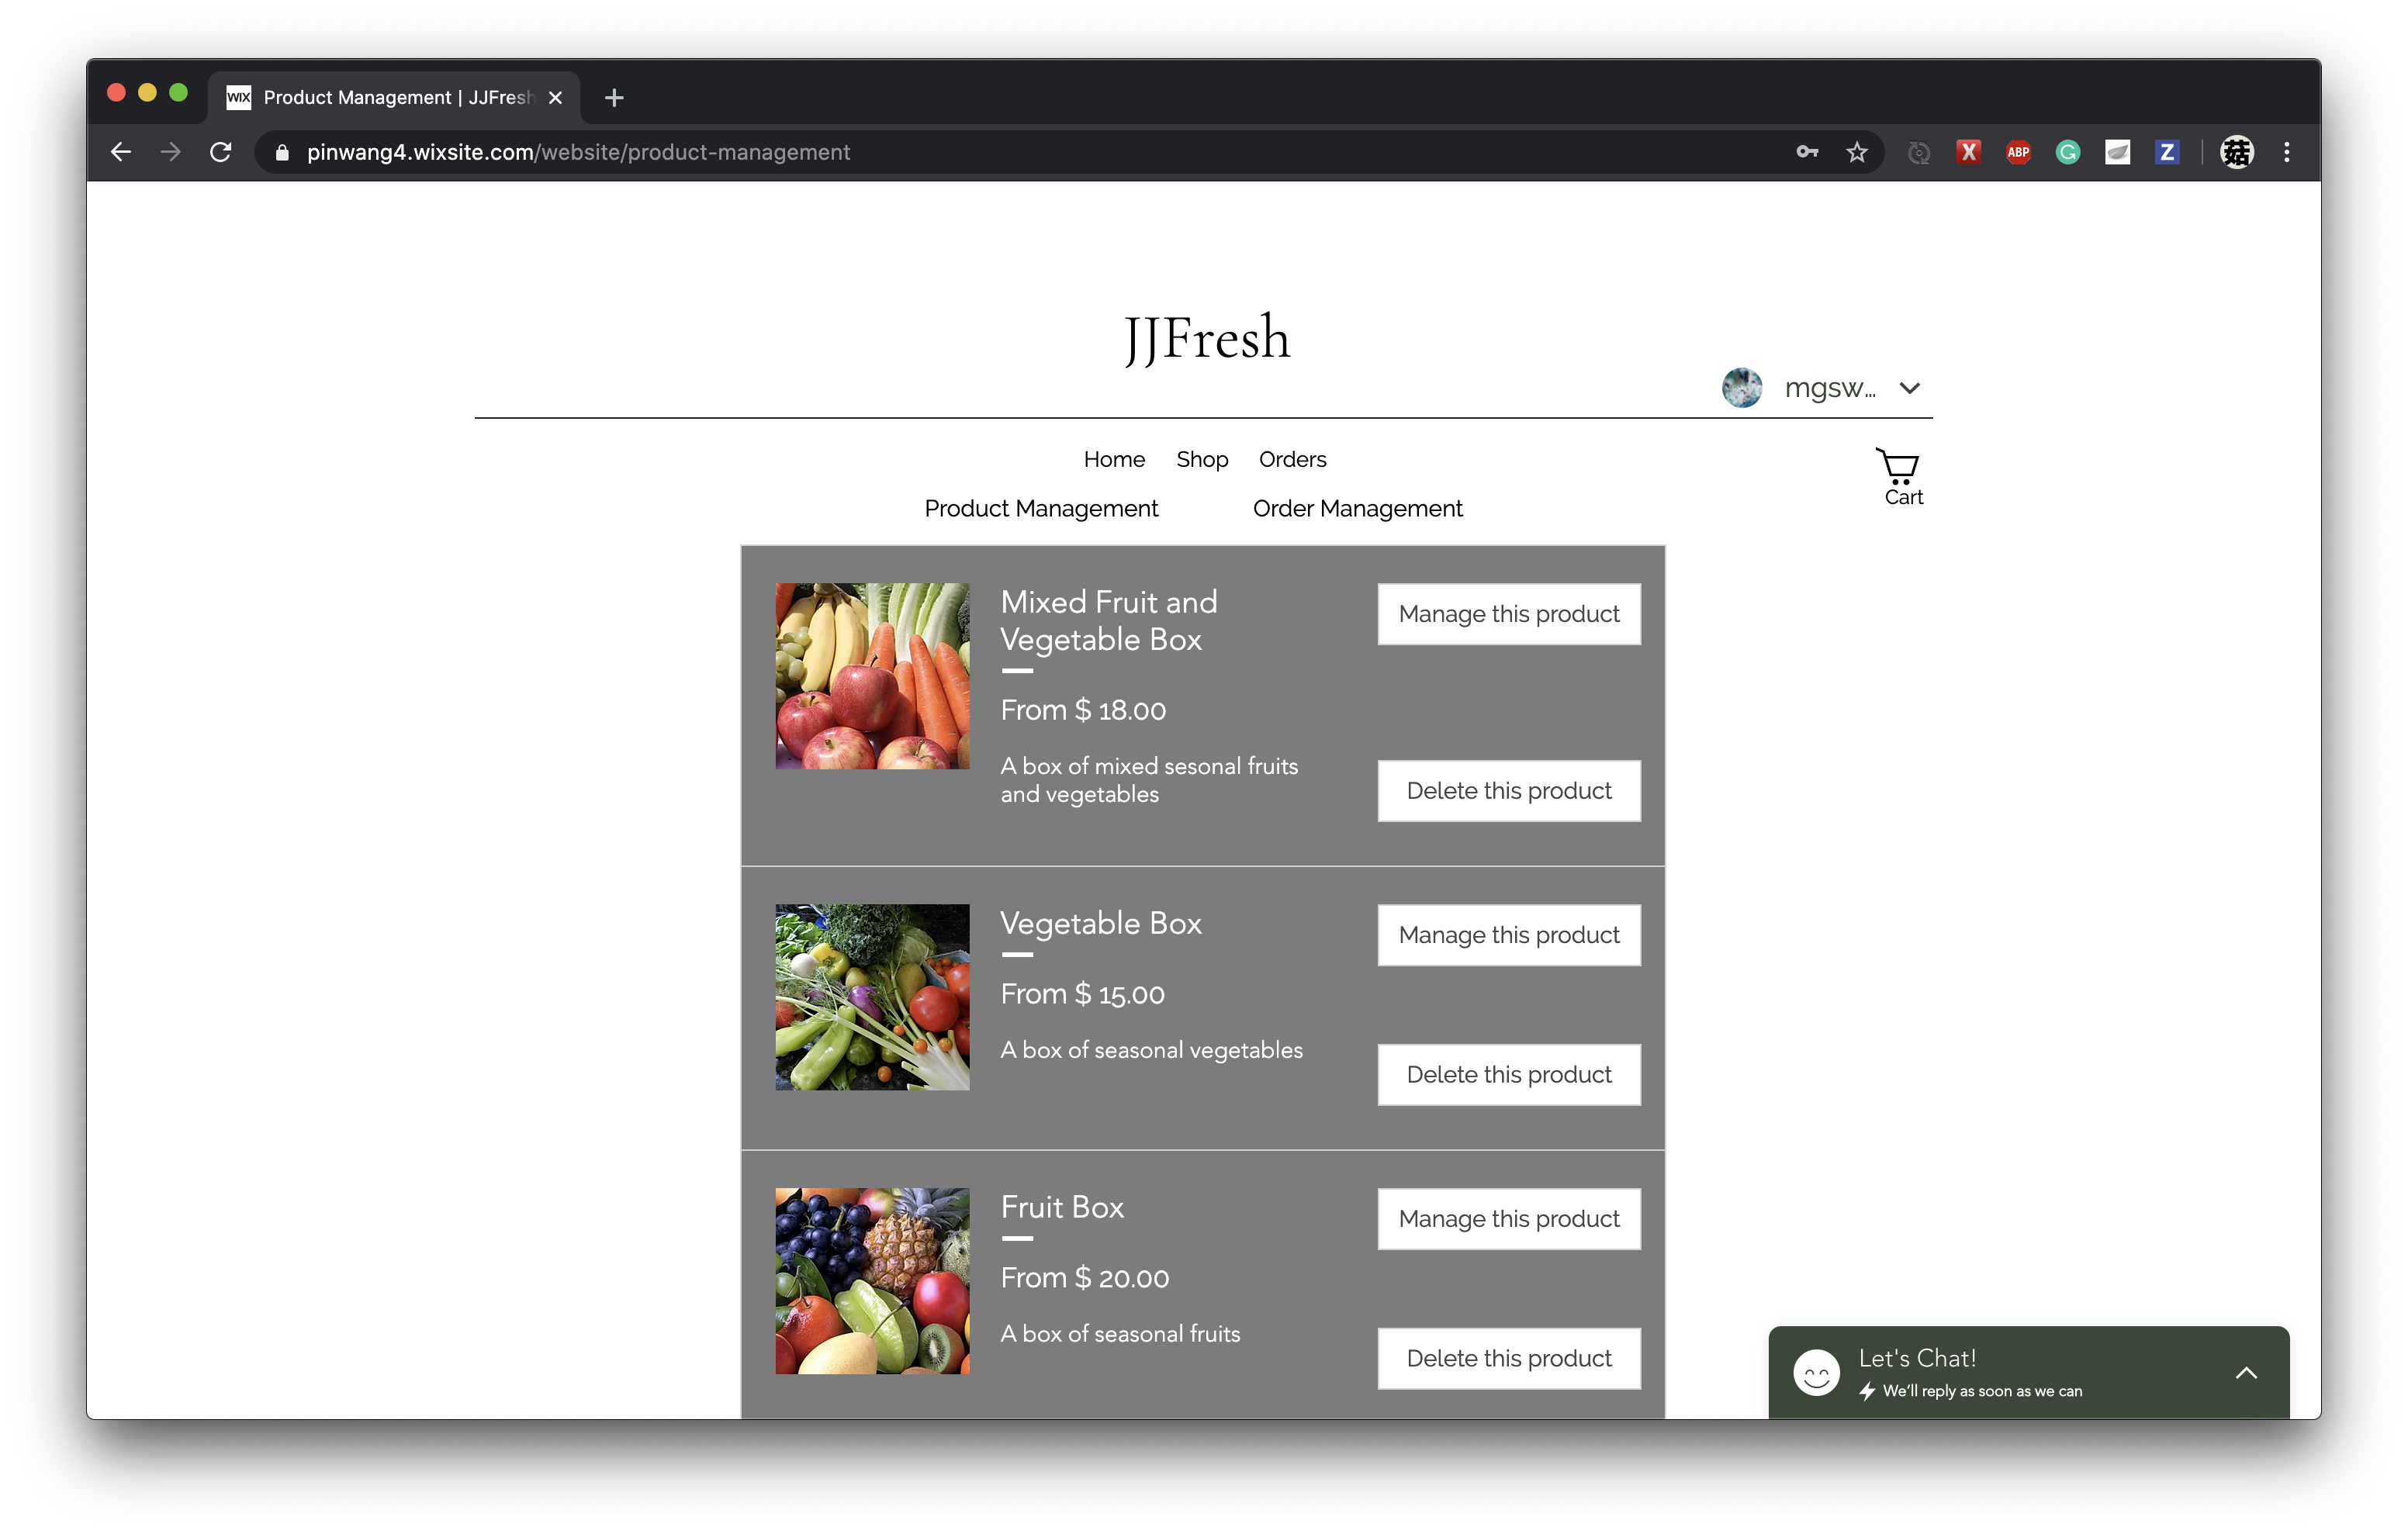
\includegraphics[width=\textwidth]{Figures/adminProduct.png}
\caption{Screenshot of product management}
\label{fig:adminProduct}
\end{figure}

\clearpage
\section*{Admin can manage the orders}
This page can be entered by click ‘Order Management’. Jess and James can manage all the orders in this page with an admin account. In each order, there is a status of order. Click the status can open a drop-down menu, which contains order placed, order confirmed, delivery completed and order canceled. Admin can adjust the status of order by click ‘Update Status’ after selecting the appropriate status.
\begin{figure}[htp]
\centering
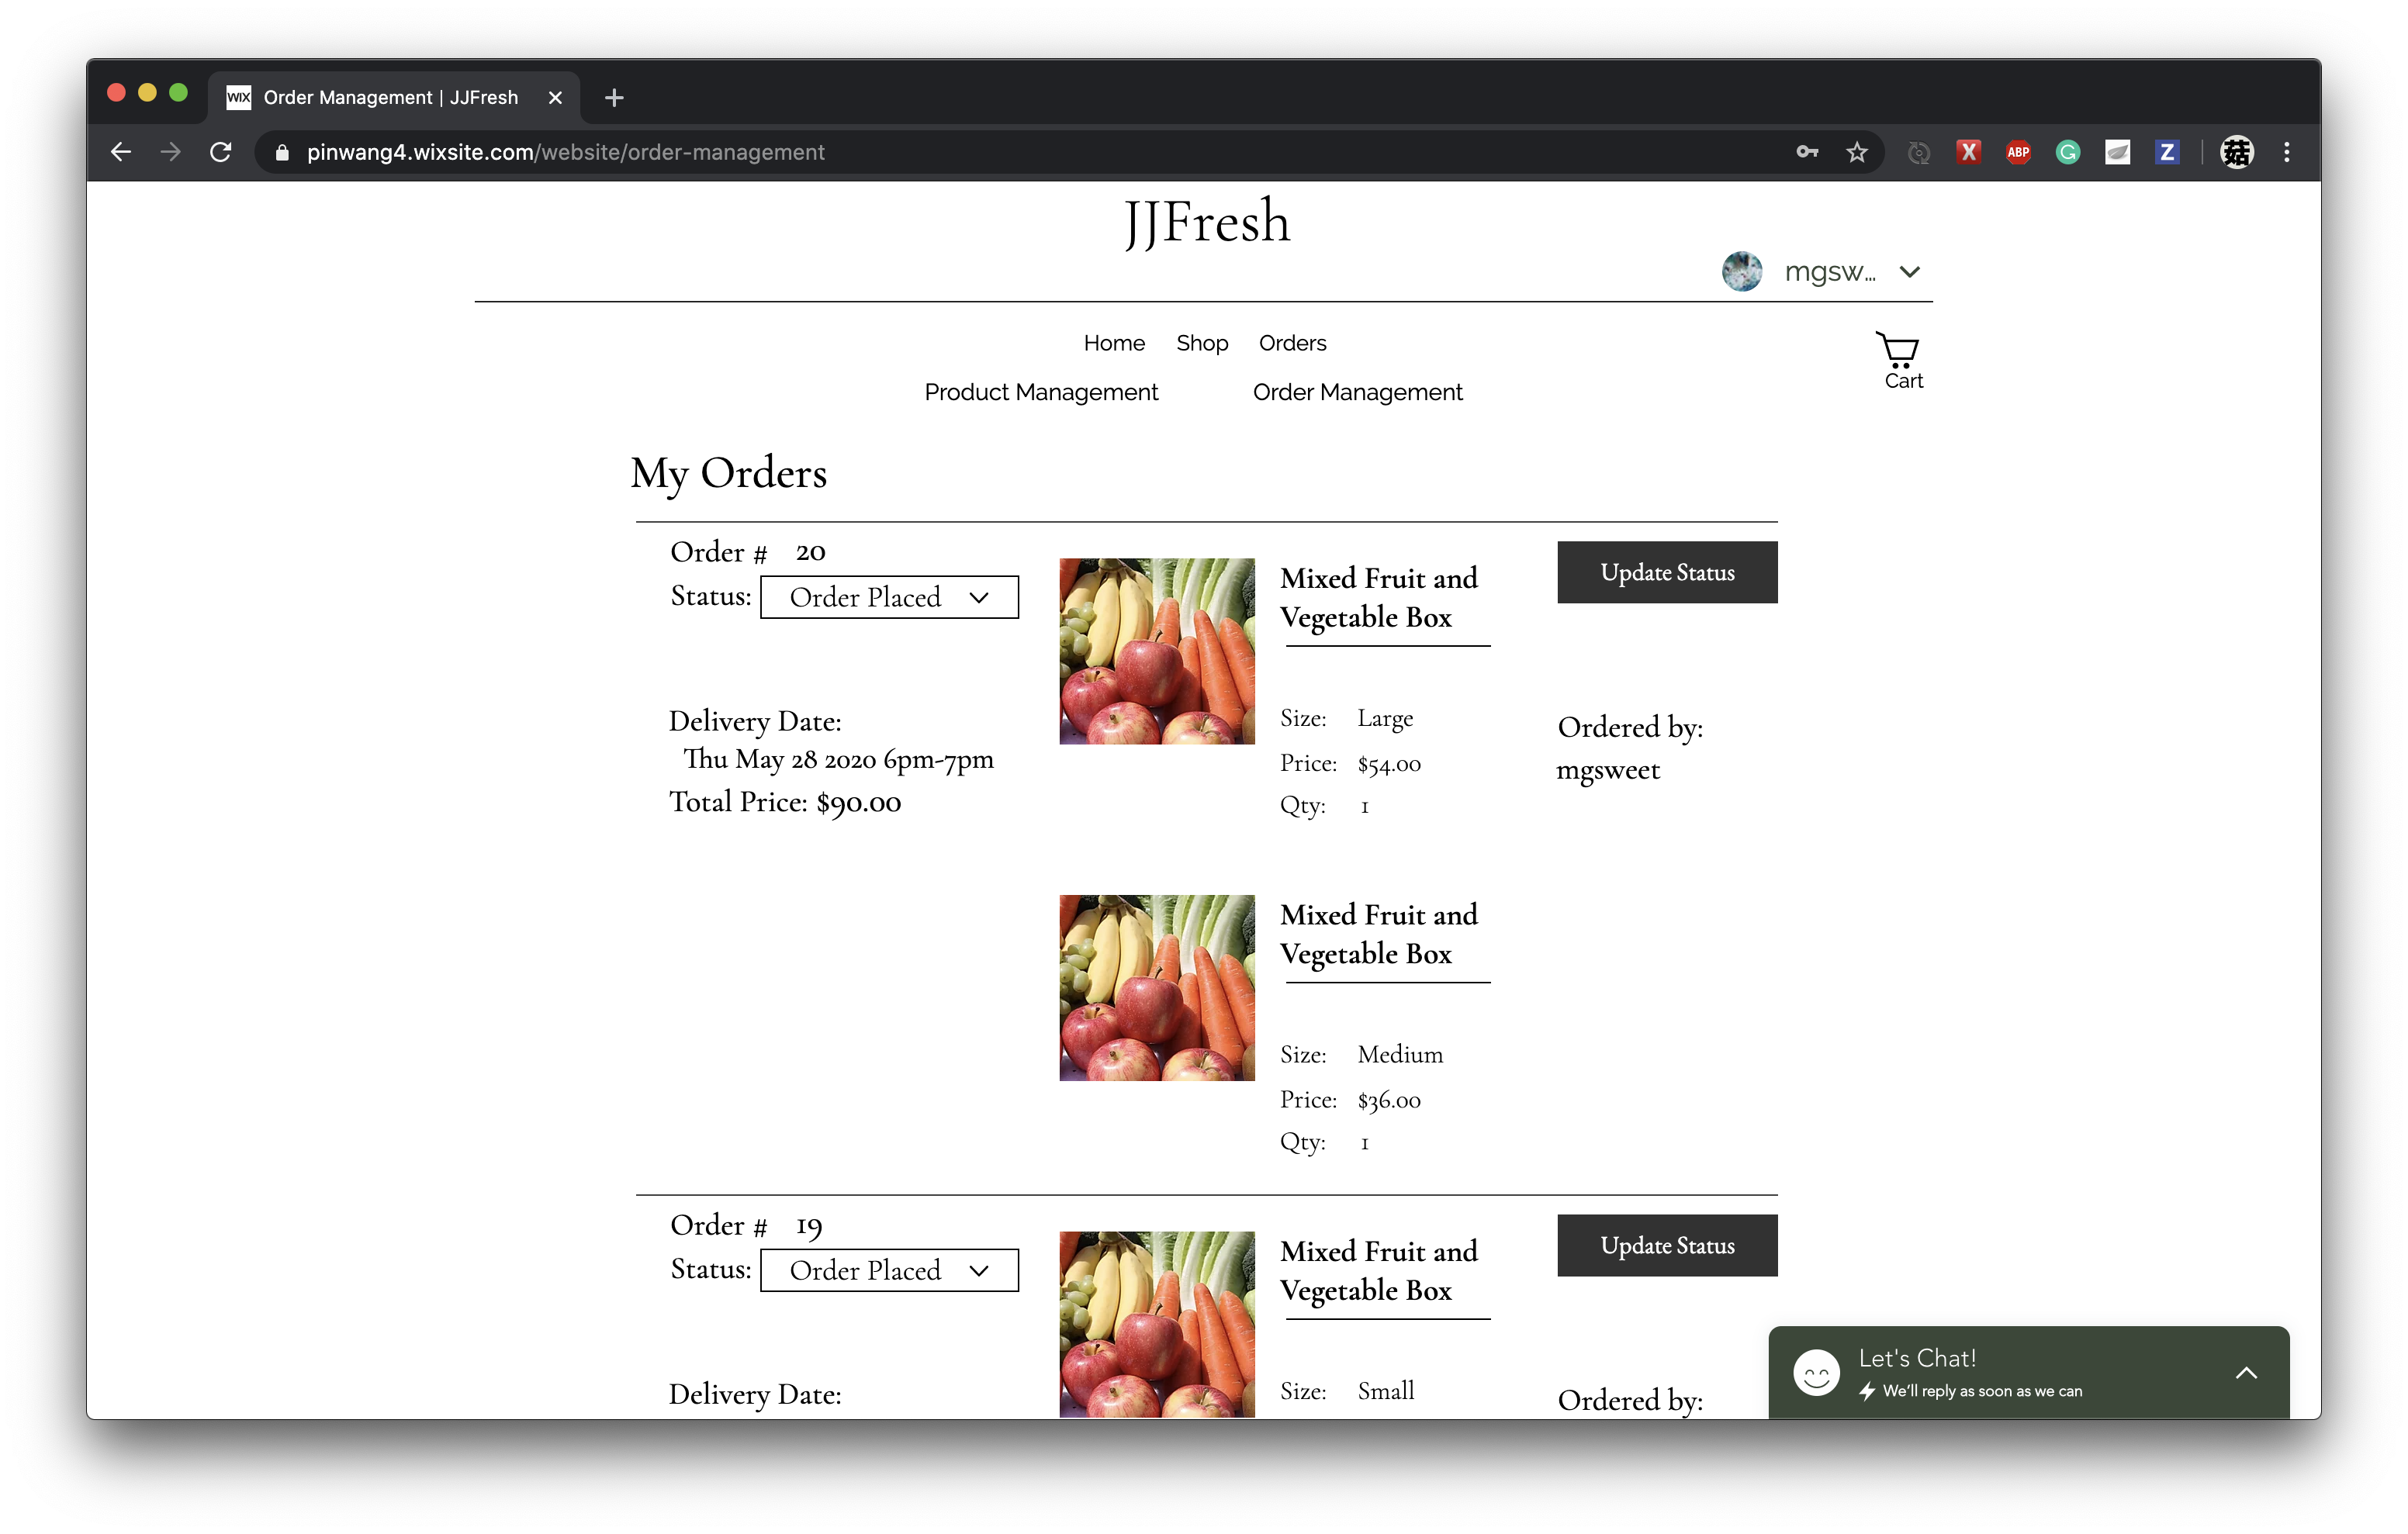
\includegraphics[width=\textwidth]{Figures/adminOrder.png}
\caption{Screenshot of order management}
\label{fig:adminOrder}
\end{figure}

